\documentclass[a4paper,10pt]{article}
\usepackage[utf8]{inputenc}
\usepackage{lipsum}
\usepackage[section]{placeins}
\usepackage{listings,xcolor}
\usepackage{enumerate}
\usepackage{booktabs}
\usepackage{vhistory}
\usepackage{graphicx}
\usepackage{placeins}
\usepackage{amsmath}
\usepackage{float}
\usepackage{fixltx2e}
\usepackage{rotating}
\usepackage{afterpage}
\usepackage{color}
\usepackage[showframe=false]{geometry}
\usepackage{changepage}
\setcounter{tocdepth}{3}
\setcounter{secnumdepth}{3}
\title{Project Plan Document}
\author{Joan Ficapal Vila (876805), Nicolò Vendramin (879113)}
\date{\today\\v1.0}
\begin{document}
  \pagenumbering{Roman}
  \begin{figure}[t]
  \centering
    
\includegraphics[scale=0.3]{Resources/logoPolimi.png}
  \end{figure}
  \thispagestyle{empty}
  \maketitle
  \newpage
  \begin{versionhistory}
    \vhEntry{0.1}{18.01.17}{N and J}{Initiated the document}
    \vhEntry{0.2}{18.01.17}{N and J}{Writing the introduction}
    \vhEntry{0.3}{19.01.17}{N and J}{Work to define the outline to be followed for Function Points and Cocomo}
    \vhEntry{0.4}{19.01.17}{N}{Starting with function points evaluation}
    \vhEntry{0.5}{19.01.17}{J}{Starting with COCOMO analysis}
    \vhEntry{0.6}{20.01.17}{N and J}{Meeting for common revision}
    \vhEntry{0.7}{20.01.17}{N}{Concluded work on Function points}
    \vhEntry{0.8}{21.01.17}{J}{Concluded work on COCOMO}
    \vhEntry{0.9}{21.01.17}{N and J}{Schedule planning}
    \vhEntry{0.10}{21.01.17}{N}{Risk Management}
    \vhEntry{0.11}{22.01.17}{J}{Resource Management}
    \vhEntry{0.12}{22.01.17}{N and J}{Revision}
    \vhEntry{1.0}{22.01.17}{N and J}{First Release}
    \vhEntry{1.1}{23.01.17}{N and J}{Small fixes}
    
    
    

  \end{versionhistory}
  \paragraph{Hours of work}
  \begin{description}
    \item[$\bullet$] Joan Ficapal Vila : 20 hours
    \item[$\bullet$] Nicolò Vendramin : 20 hours
   \end{description}
   \newpage
  \tableofcontents
  \newpage
  \pagenumbering{arabic}

\maketitle
\section{Introduction}
\subsection{Purpose and Scope}
\paragraph{} This document is the Project Plan Document for the PowerEnjoy application. The main purpose of the following document is to estimate the complexity
of the project in order to assist the project leader in the activity of estimations of costs and efforts. 
The first part of the document will be dedicated to the estimation of the size of the project using the function points method, together with a cost and effort
estimation done following the COCOMO approach.  \\
In the second part of the document we are going to propose a possible schedule for the activities that compose the project, from the elicitation and identification
of the requirements to the implementation and testing activities. After that the document will present a possible scheme for the allocation of the 
human resources available for the project to the different activities composing the schedule, and at last an analysis concerning the possible 
risks that project could face in the different stages of develpment.
  
\subsection{Definitions, Acronyms and Abbreviations}
  \subsubsection{Acronyms}
  \begin{description}
    \item[$\bullet$] \textbf{FP:} Funtion Points. Is a method to estimate the dimension of the source code needed to implement
    the functionalities of a program.
    \item[$\bullet$] \textbf{SLOC:} Source Lines of Code. Lines of source code. The number of line needed for the implementation of
    a program.
    \item[$\bullet$] \textbf{API:} Access Point of Interface. APIs are the methods exposed by a software product to be used by other 
    softwares.
    \item[$\bullet$] \textbf{ELF:} External Logical File. One of the function types used in the Function Points method.
    \item[$\bullet$] \textbf{ILF:} Internal Logical File. One of the function types used in the Function Points method.
    \item[$\bullet$] \textbf{EI:} External Input. One of the function types used in the Function Points method.
    \item[$\bullet$] \textbf{EO:} External Output. One of the function types used in the Function Points method.
    \item[$\bullet$] \textbf{EQ:} External inQuiries. One of the function types used in the Function Points method.
    \item[$\bullet$] \textbf{COCOMO II:} COnstructive COst MOdel. Is a model that allows to estimate the cost, effort and schedule when planning
    a new software development activity.
  \end{description}
  \subsubsection{Definitions}
   \begin{description}
   \item[$\bullet$] \textbf{Unit Testing:} With unit testing is meant that activity that make sure that every basic unit that composes the software is correctly 
   working as expected. With unit we indicate the smaller atom of which the software is composed. In case of a Java program we can assume Classes as units.
   \item[$\bullet$] \textbf{Integration Testing:} With integration testing is meant that phase 
   of software testing in which individual modules are tested together as a group.
   
   \end{description}
\subsection{Reference Documents}
Here we attached the list of all the documents that are kept as references in the writing of this document.
\begin{description}
    \item[$\bullet$] Templates provided at lesson.
    \item[$\bullet$] Slides of the course.
    \item[$\bullet$] COCOMO II official documentation.
    \item[$\bullet$] Function Points method documentation.
  \end{description}
 \newpage
 
\section{Project size, cost and effort estimation}
\subsection{Size estimation: function points}
For the estimation of the project size we chose to use the method of the function points. This method has been defined in 1975 by Allan Albrecth and is 
based on the assumption the dimension of any software product can be estimated basing on the functionalities that it has to offer. In particular
basing on the combinations of some particular software characteristics (Data structures, inputs and outputs, inquiries and external services)
to whom are associated specific weights, is possible to estimate the dimension of the software to be developed. The steps that must be followed to apply 
this method are mainly the identification and classification of the different function points, followed by the weighted sum of them which is an
estimator of the number of lines of code needed to implement the identified functional points. The number of functional points to
assign to each element of a certain function type have been derived from the analysis of real project
developed in the past and condensed in the following tables that we attach at the end of the paragraph.
  \bigskip
  \begin{figure}[h]
  \centering
    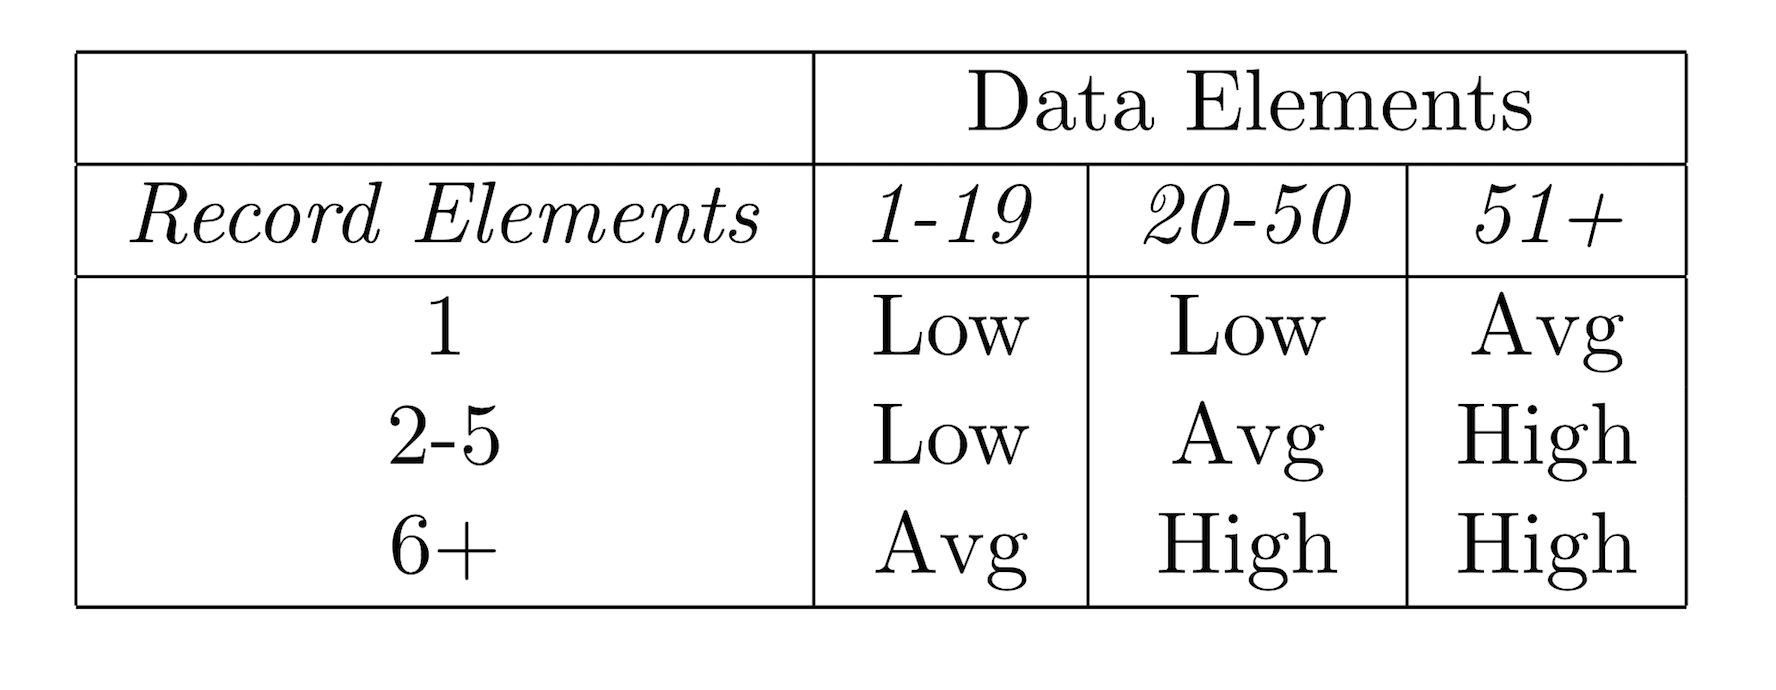
\includegraphics[scale=0.3]{Resources/ilf.png}
    \caption{Internal Logic Files, Complexity Weight Assignment}
  \end{figure}
  \begin{figure}[h]
  \centering
    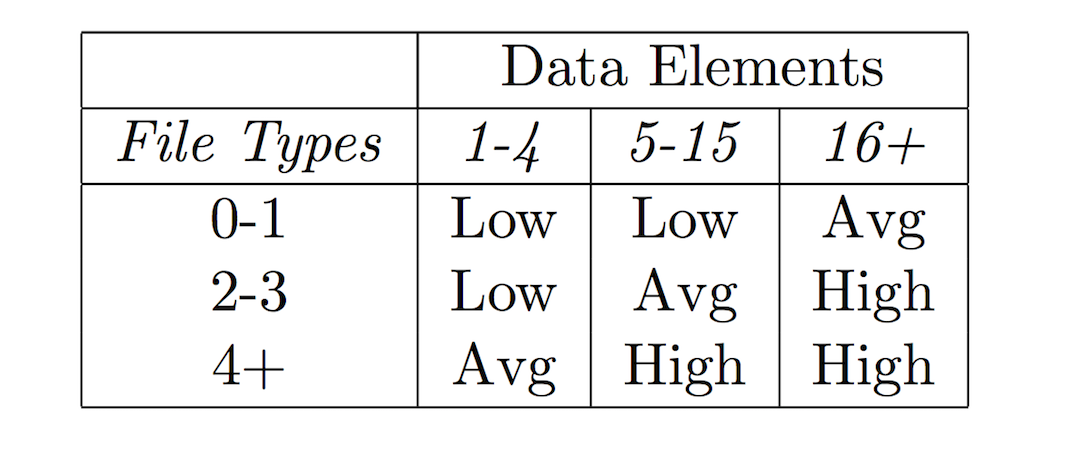
\includegraphics[scale=0.46]{Resources/einpu.png}
    \caption{Exernal Input, Complexity Weight Assignment}
  \end{figure}
  \begin{figure}[h]
  \centering
    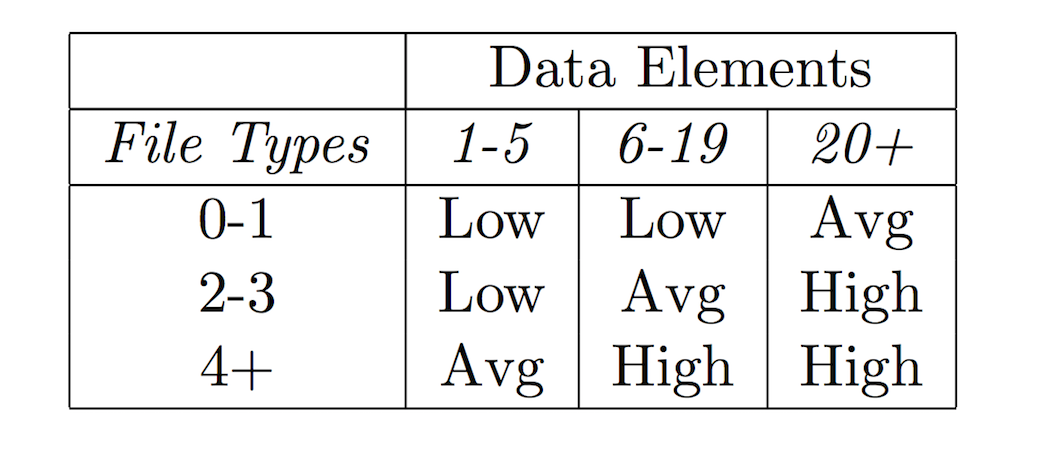
\includegraphics[scale=0.46]{Resources/eoei.png}
    \caption{External Output and Inquiries, Complexity Weight Assignment}
  \end{figure}
  \begin{figure}[h]
  \centering
    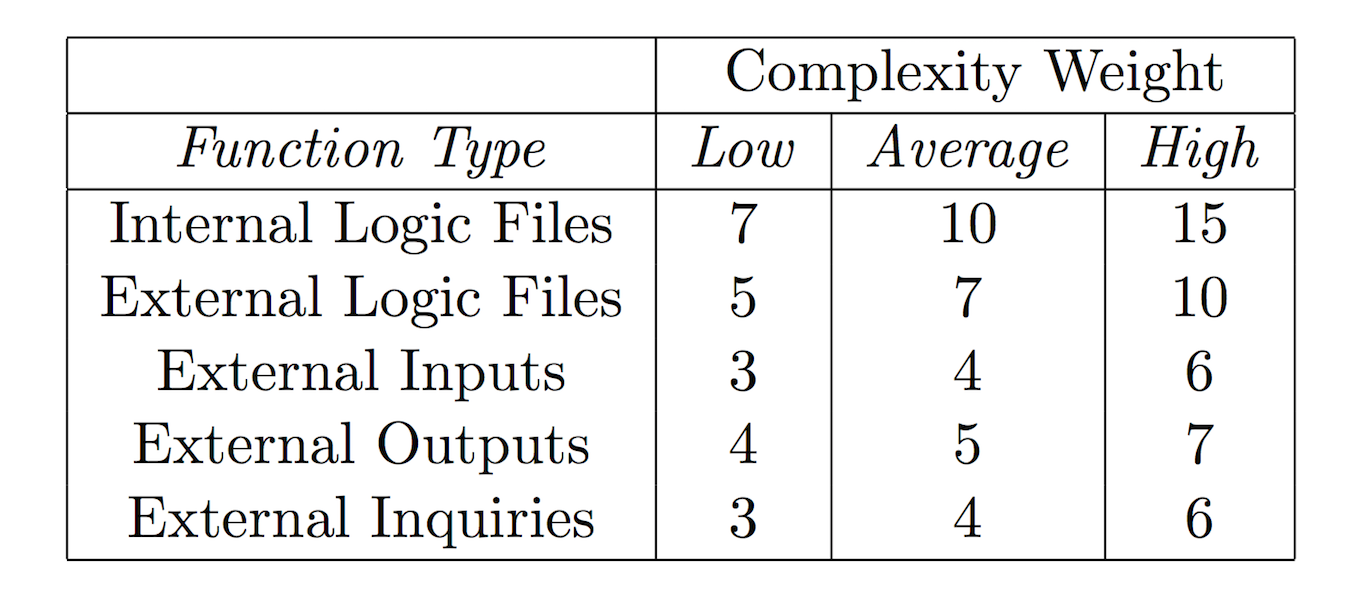
\includegraphics[scale=0.46]{Resources/complwe.png}
    \caption{Complexity Weight translation to Function Points, for each Function Type}
  \end{figure}
  \FloatBarrier
\subsubsection{Internal Logic Files (ILFs)} Internal logic files is the first type of function points and it is the one that is that represents the 
set of data that are used and managed by the application. In the case of our application the data that are internally managed by the application 
are the ones stored in the internal database about: Clients, Areas, Cars, Service, Bill, Cookie Session.
\\Client are stored in a table, with an unique index that is used in a second table to associate every client id to the password.
A third table stores informations about the areas (area id, reference adress, type of area). In another table
the points that form the limits for the polygon that identifies every area are stored in association to the id of the correspondin area.
An additional table is dedicated to the informations about the cars that form the system and in particular it contains the Plate, the location,
the state of the car (Booked, Free or inRide), the boolean that represent wether the engine is on or off, the number of occupied seats and the 
status of the battery. Services are stored in two different tables depending on wether they are bookings or rides.
In both cases the key is given by the combination of car id, client id and timestamp 
followed by the different attributes of the service itself (that vary depending on the type of service).
The bills are stored in a table where to every service id is attributed the corresponding amount of money charged to the user and the timestamp 
of the invocation of the billing system. Cookie sessions are stored in a table composed of three attributes: cookie session, 
user id (optional), and timestamp.
A special table is dedicated to store the booking timers: this table is made up of associations between service id and timestamps.
  \begin{figure}[h]
  \centering
    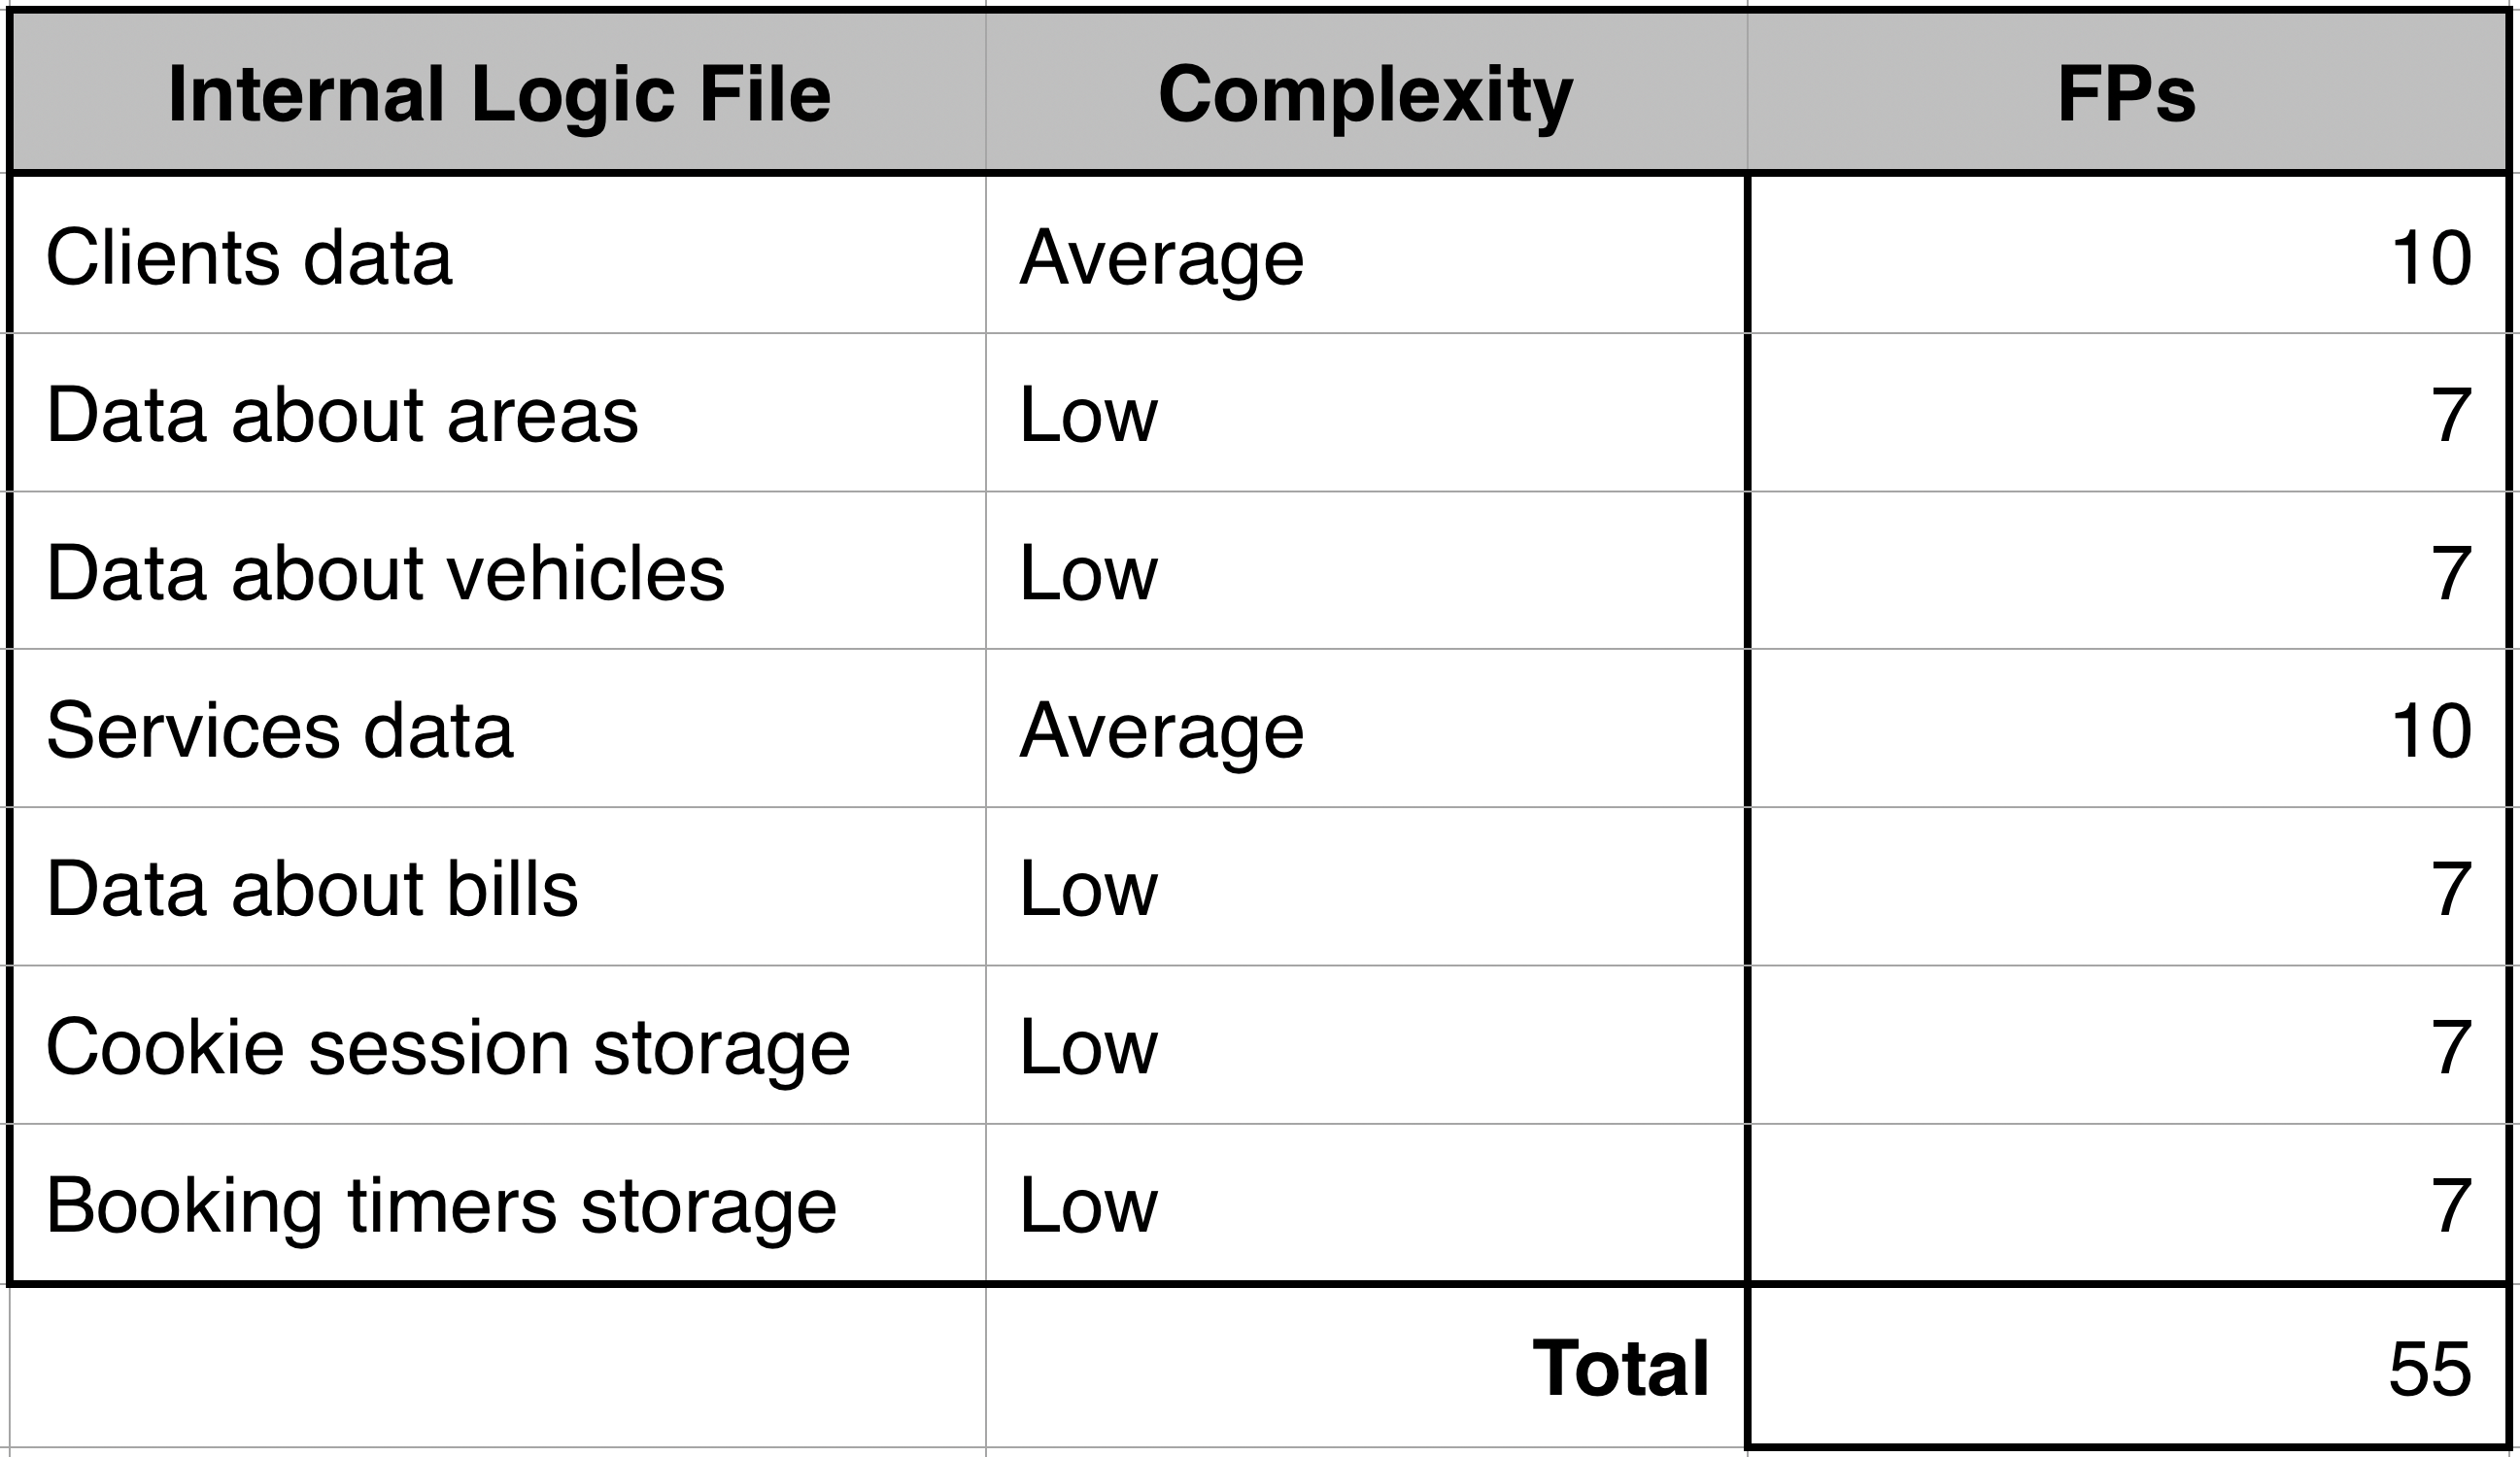
\includegraphics[scale=0.2]{Resources/intlogic.png}
    \caption{Internal Logic Files, Resume Table}
  \end{figure}
\subsubsection{External Logic Files (ELFs)} The second functional type is External Interface Files amd represents all those source of 
data external to the application its users. In the PowerEnjoy application the impact of External Interface Files is quite important
since the main source of data for the system is the existing systems that handles the data concerning the operation of the application.
The main interactions are related to the vehicles rented by the service. The information about them is not queried by our system directly, 
instead is updated by the existing system that after every relevant change updates the state of the private database of the 
PowerEnjoy application. Some operations in the interaction with this system return data that must be processed and used by the application:
in particular those interactions are the one in which the Login, Register, ShowAccountInfo, ShowCarDetails and ShowVehicles apis of the
existing system. Since the elaboration of the returned data has a low complexity we assign to each of this external interface files 10 FPs,
so that summing them up we obtain a total of 50 FPs.
  \begin{figure}[h]
  \centering
    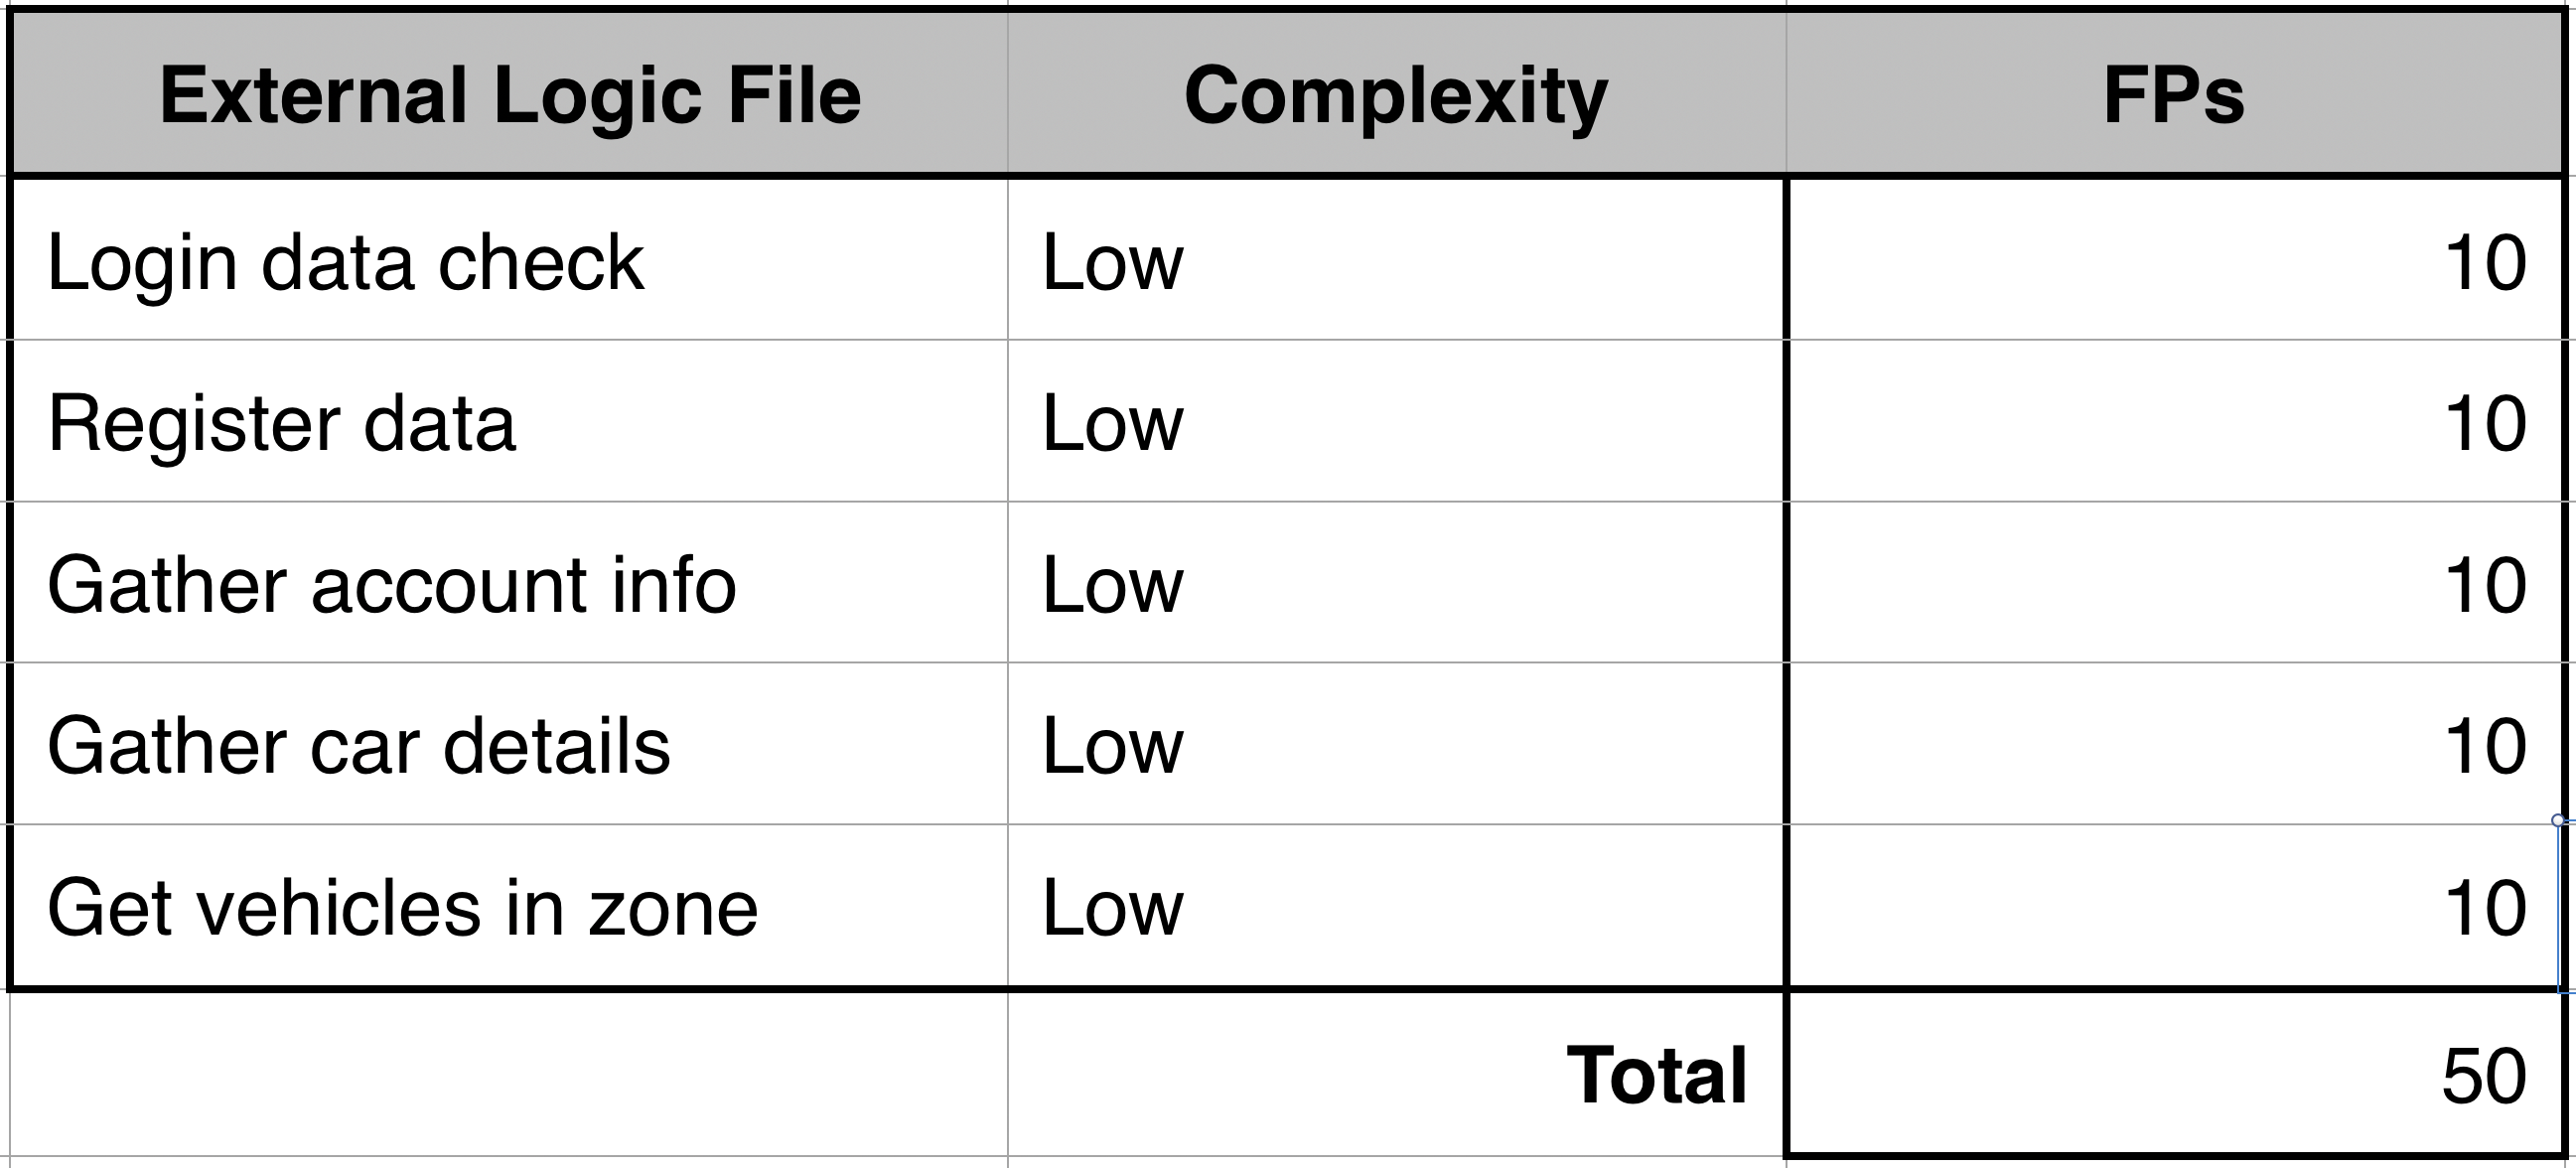
\includegraphics[scale=0.2]{Resources/exlogic.png}
    \caption{External Logic Files, Resume Table}
  \end{figure}
\subsubsection{External Inputs (EIs)} External Inputs is that function type that deals with operation that has to elaborate data coming from
the external environment.
The PowerEnjoy application supports inputs within different interactions with the two types of user
that can use the application. All the inputs coming from users must be processed by the Request manager and since
this component does not elaborate the inputs but only invoke the right components in the controller, we omit it in the following 
description. \\All people accessing the platform can interact through:
\begin{description}
    \item[$\bullet$] Registration: This simple operations, at the level of the business logic components only involve the activity
    of the Login/ Register Manager. For this reason it can be considered as simple and it only account for
    3 FPs.
  \end{description}
 While the interactions in which the system receives data from an already registered user, are the ones belonging to the following list:
 \begin{description}
    \item[$\bullet$] Login/ Logout: This is a simple operation that interacts with the Registration/ Login Manager and DBMS. For this 
    reason it can be given a value of 6 FPs, considering 3 for each one of the two.
    \item[$\bullet$] Book car/ Cancel Booking: those operations are more complex since they require the action of The booking manager,
    the creation of records
    in the database and also an interaction with the external existing system. 
    Given their complexity we estimate for this point a total of 12 FPs equally distributed between the two operations.
    \item[$\bullet$] Open car: this operation, as it was said for the precedent one is to be considered quite complex and for this 
    reason is labeled with 5 FPs.
    \item[$\bullet$] Conclude rent: this operation is the most complex between the ones offered to the users. This requires our
    system to employ the ride manager, the price and discount manager, to work on the DBMS and to interact with the APIs exposed 
    by the external billing system. For this reason its extimated cost is considered to be 8.
  \end{description}
  \begin{figure}[h]
  \centering
    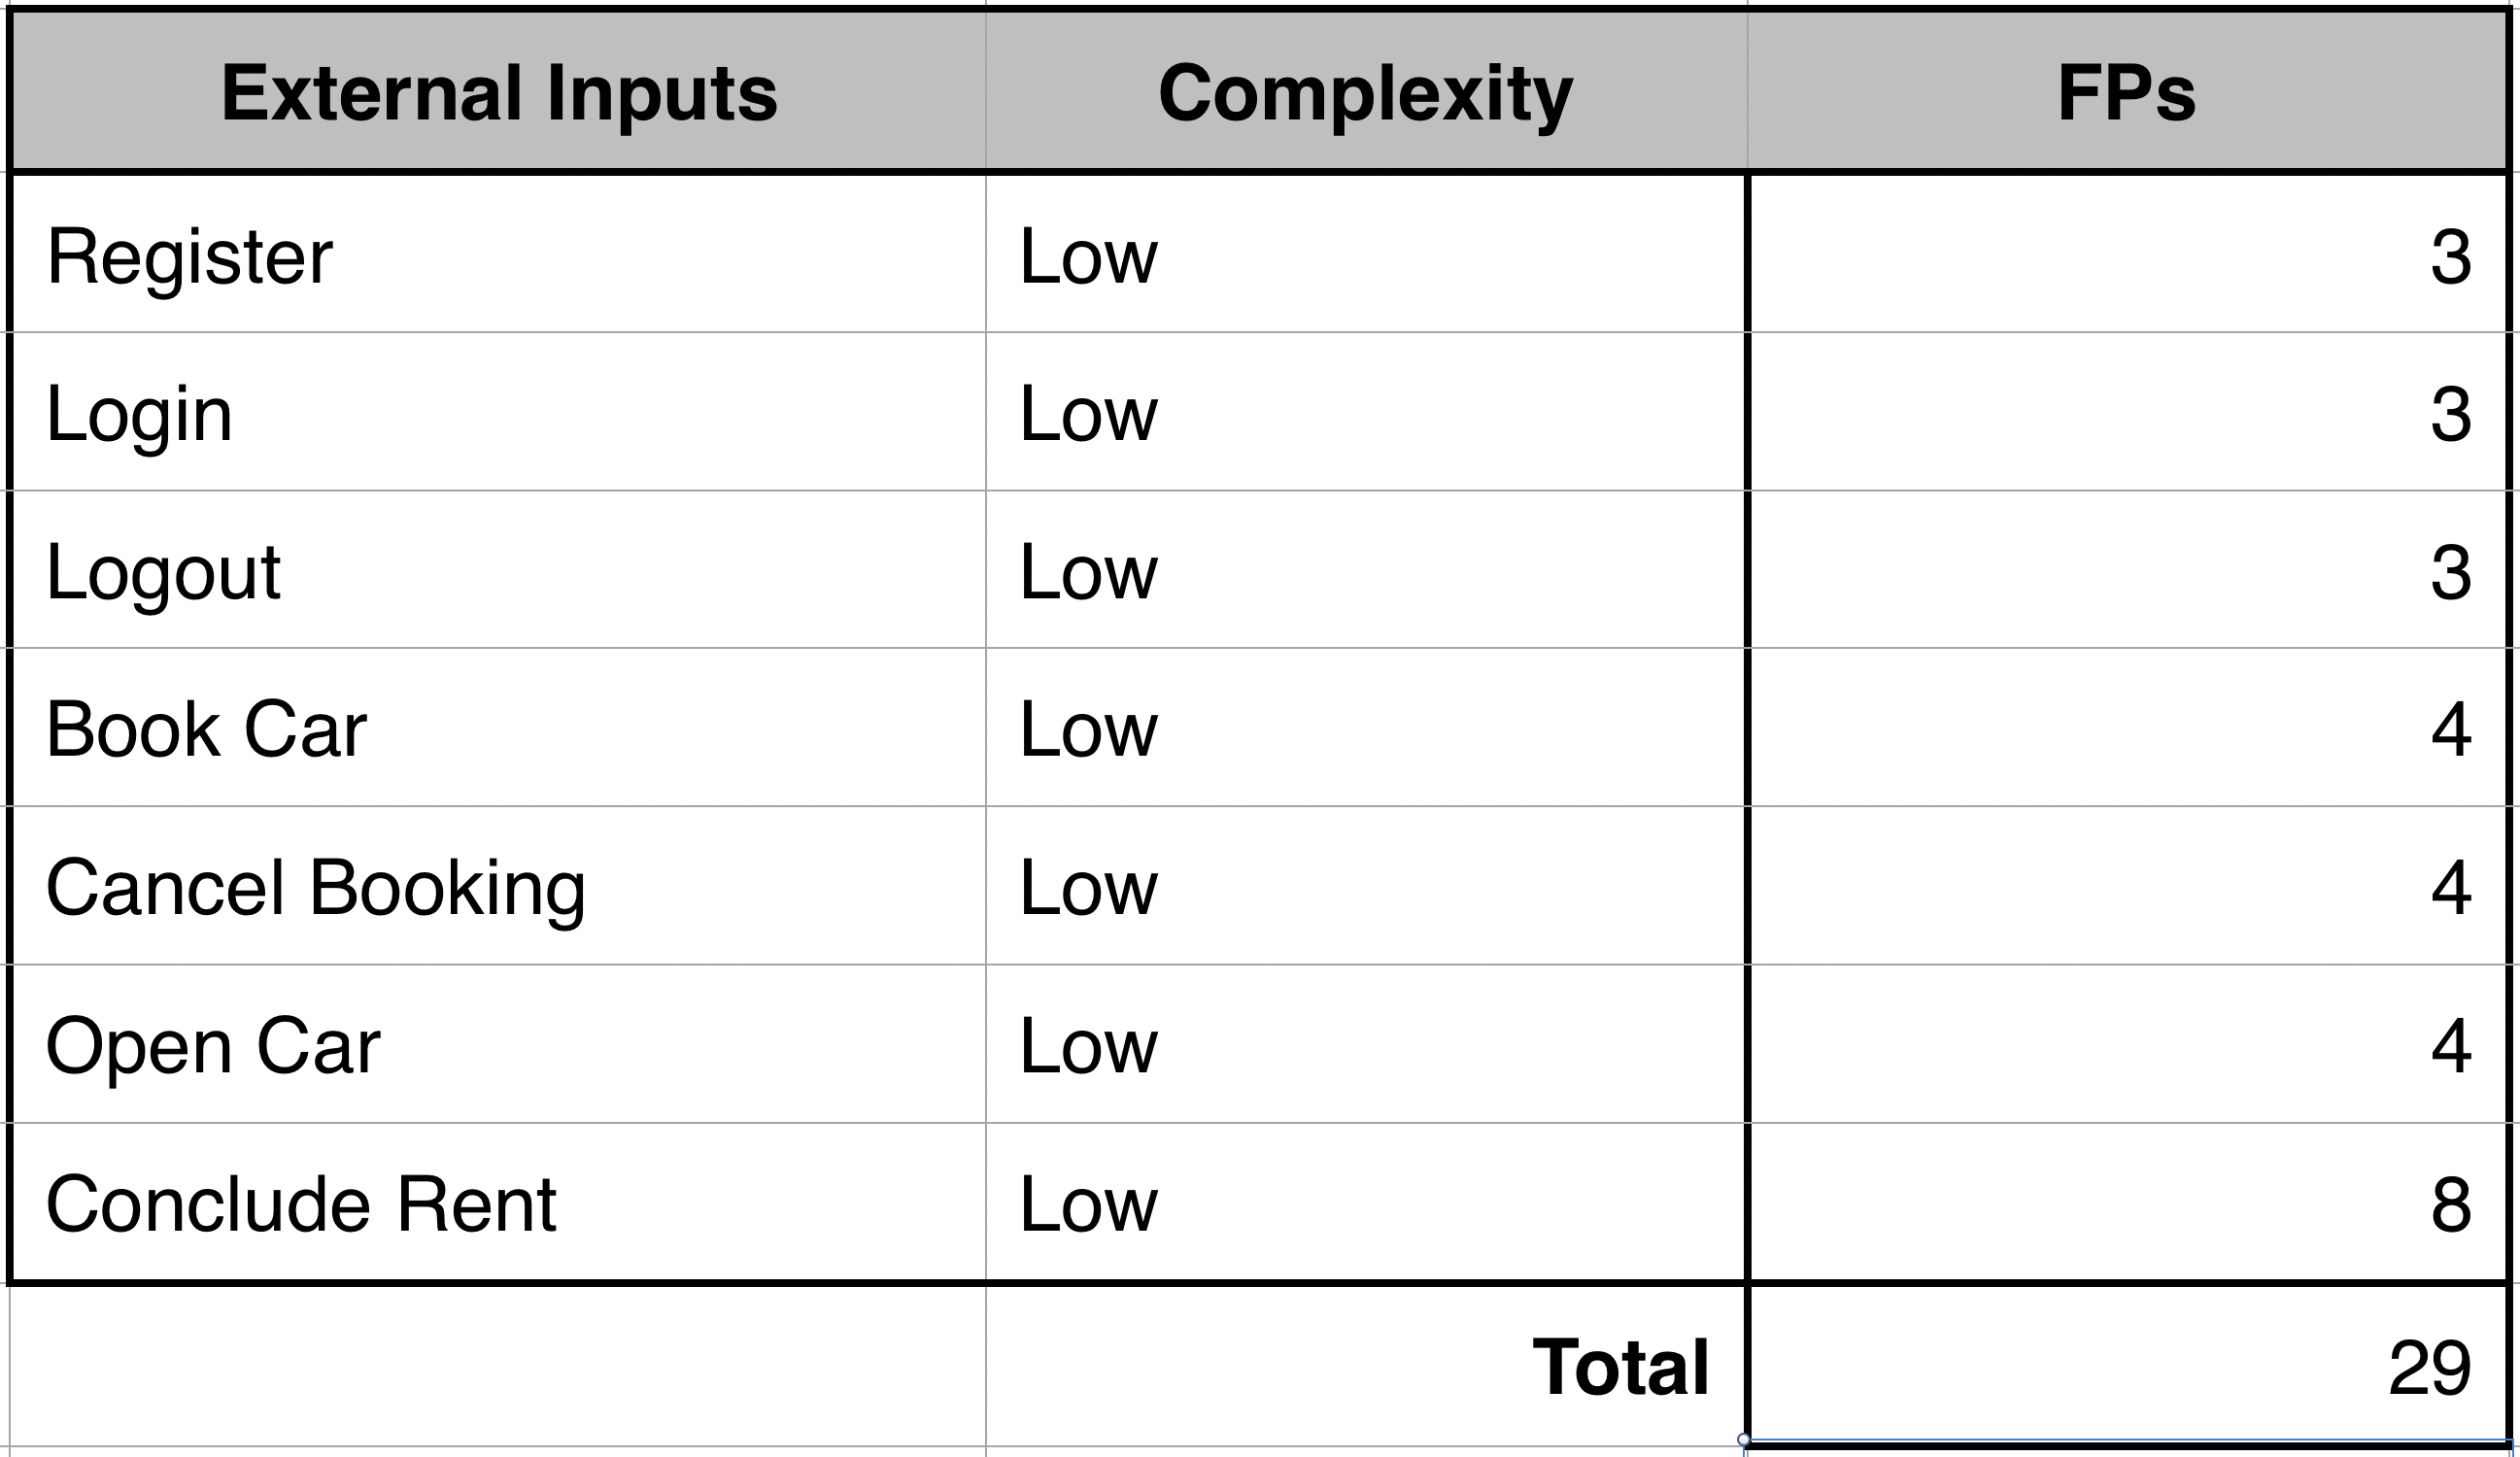
\includegraphics[scale=0.2]{Resources/exinput.png}
    \caption{External Inputs, Resume Table}
  \end{figure}
\subsubsection{External Inquiries (EQs)} The third functional type is External Inquiries and consists of all those operations
that involve both the acquisition of an input and the creation of an output. In the case of our application there are mainly
three kind of interactions that the registered user can do with the system that can be considered under this label:
     \begin{description}
    \item[$\bullet$] View cars available in one zone: this operation is quite light-weighted from the point of view of the business logic
    of the application. It involves only the resource manager and the DBMS, and it can be considered a simple inquiry. For this reason
    it is given 3 FPs.
    \item[$\bullet$] View the detailed of a specific car: this can be considered a basic operation. It is served by the resource manager 
    and involves a simple interaction with the database. According to this we give it a value of 3 FPs.
    \item[$\bullet$] View Account Details: this operations, as the ones above mentioned, is easy to handle by the system and is composed
    by a straight forward query on the database performed by the resouce manager. Seen the low complexity of the business-logic that 
    supports it, the operation is considered for a value of 3 FPs.
      \end{description}
  \begin{figure}[h]
  \centering
    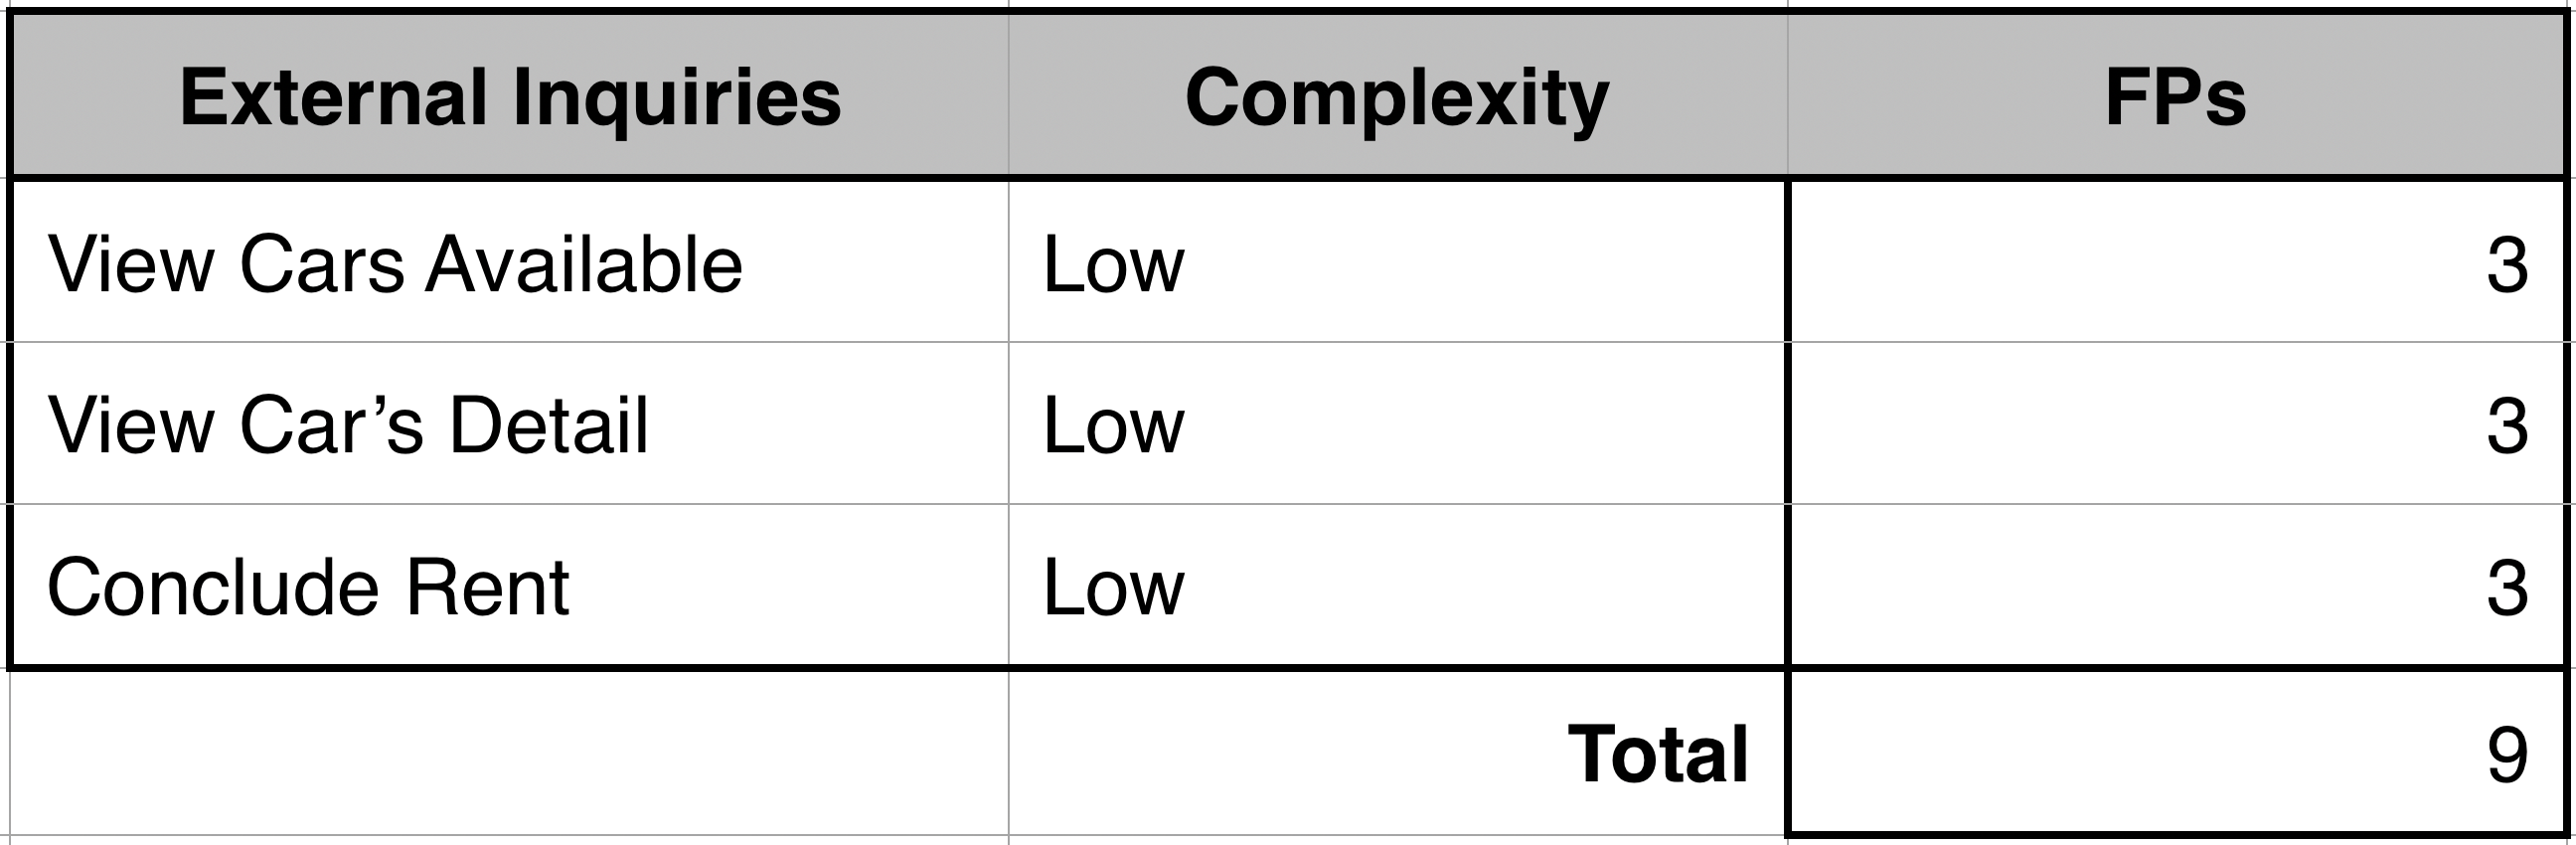
\includegraphics[scale=0.2]{Resources/inquiries.png}
    \caption{External Inquiries, Resume Table}
  \end{figure}
  \subsubsection{External Outputs (EOs)} Under the Functional Type called External Outputs, are grouped those operations in which the system generates
  data for the external environment. In the case of the PowerEnjoy, this kind of operation are served by the functionality called notify, provided
  by the request manager. Since this function is then called in many of the routines that are executed on the system we give to it a
  complexity weight of Average with a corresponding assignment of 7 function points.
  \begin{figure}[h]
  \centering
    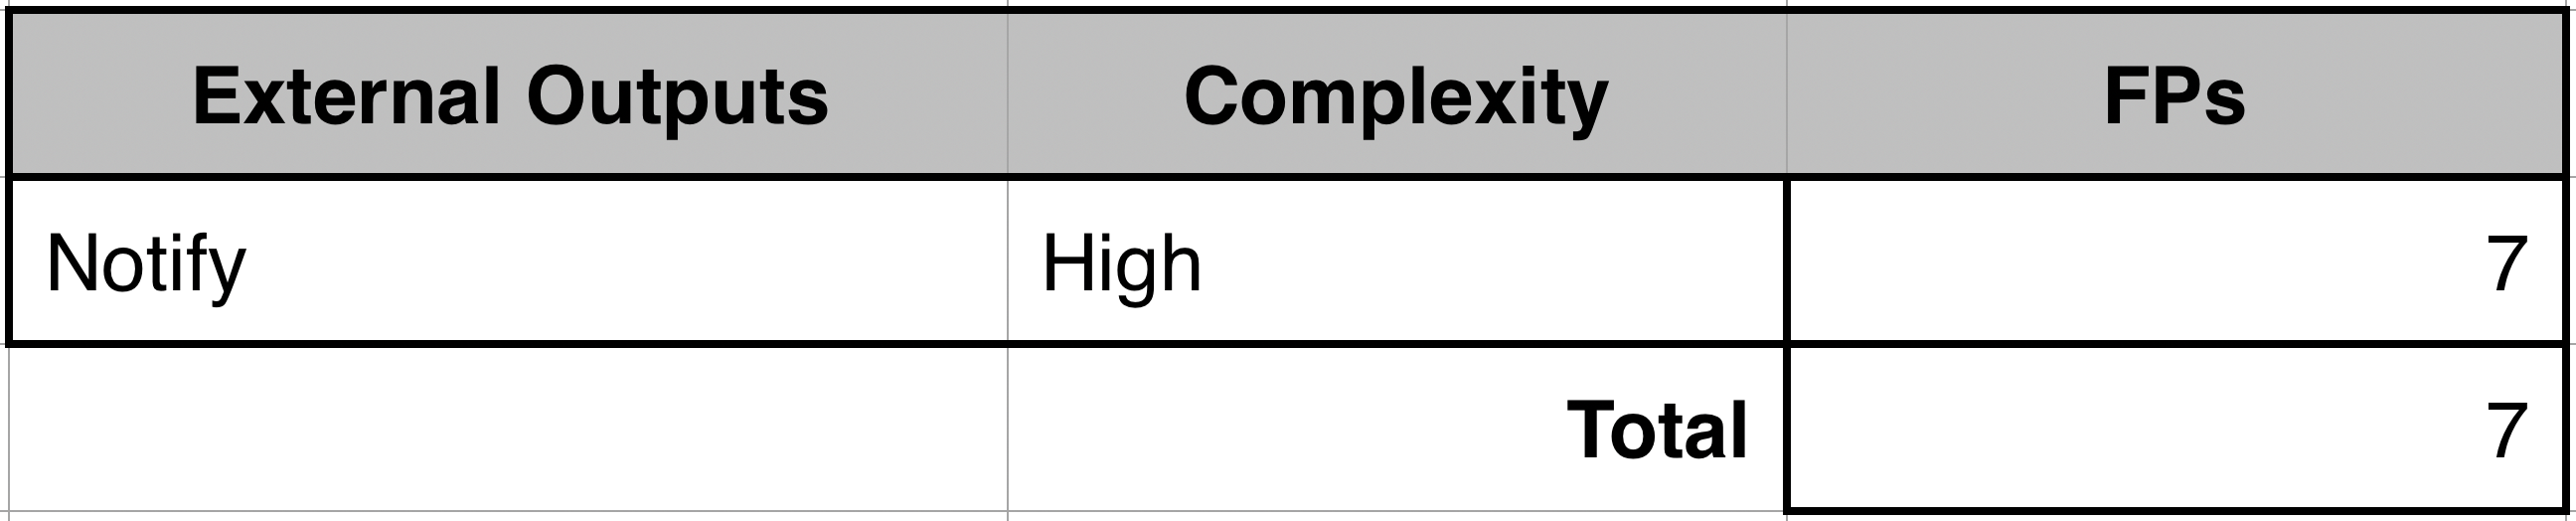
\includegraphics[scale=0.2]{Resources/outputs.png}
    \caption{External Outputs, Resume Table}
  \end{figure}
  \subsubsection{Overall Estimation} Given the above calculated complexities for each single element weighted according to
  the tables above mentioned we have now the function points of all the types. They are resumed in the following table:
    \begin{figure}[h]
  \centering
    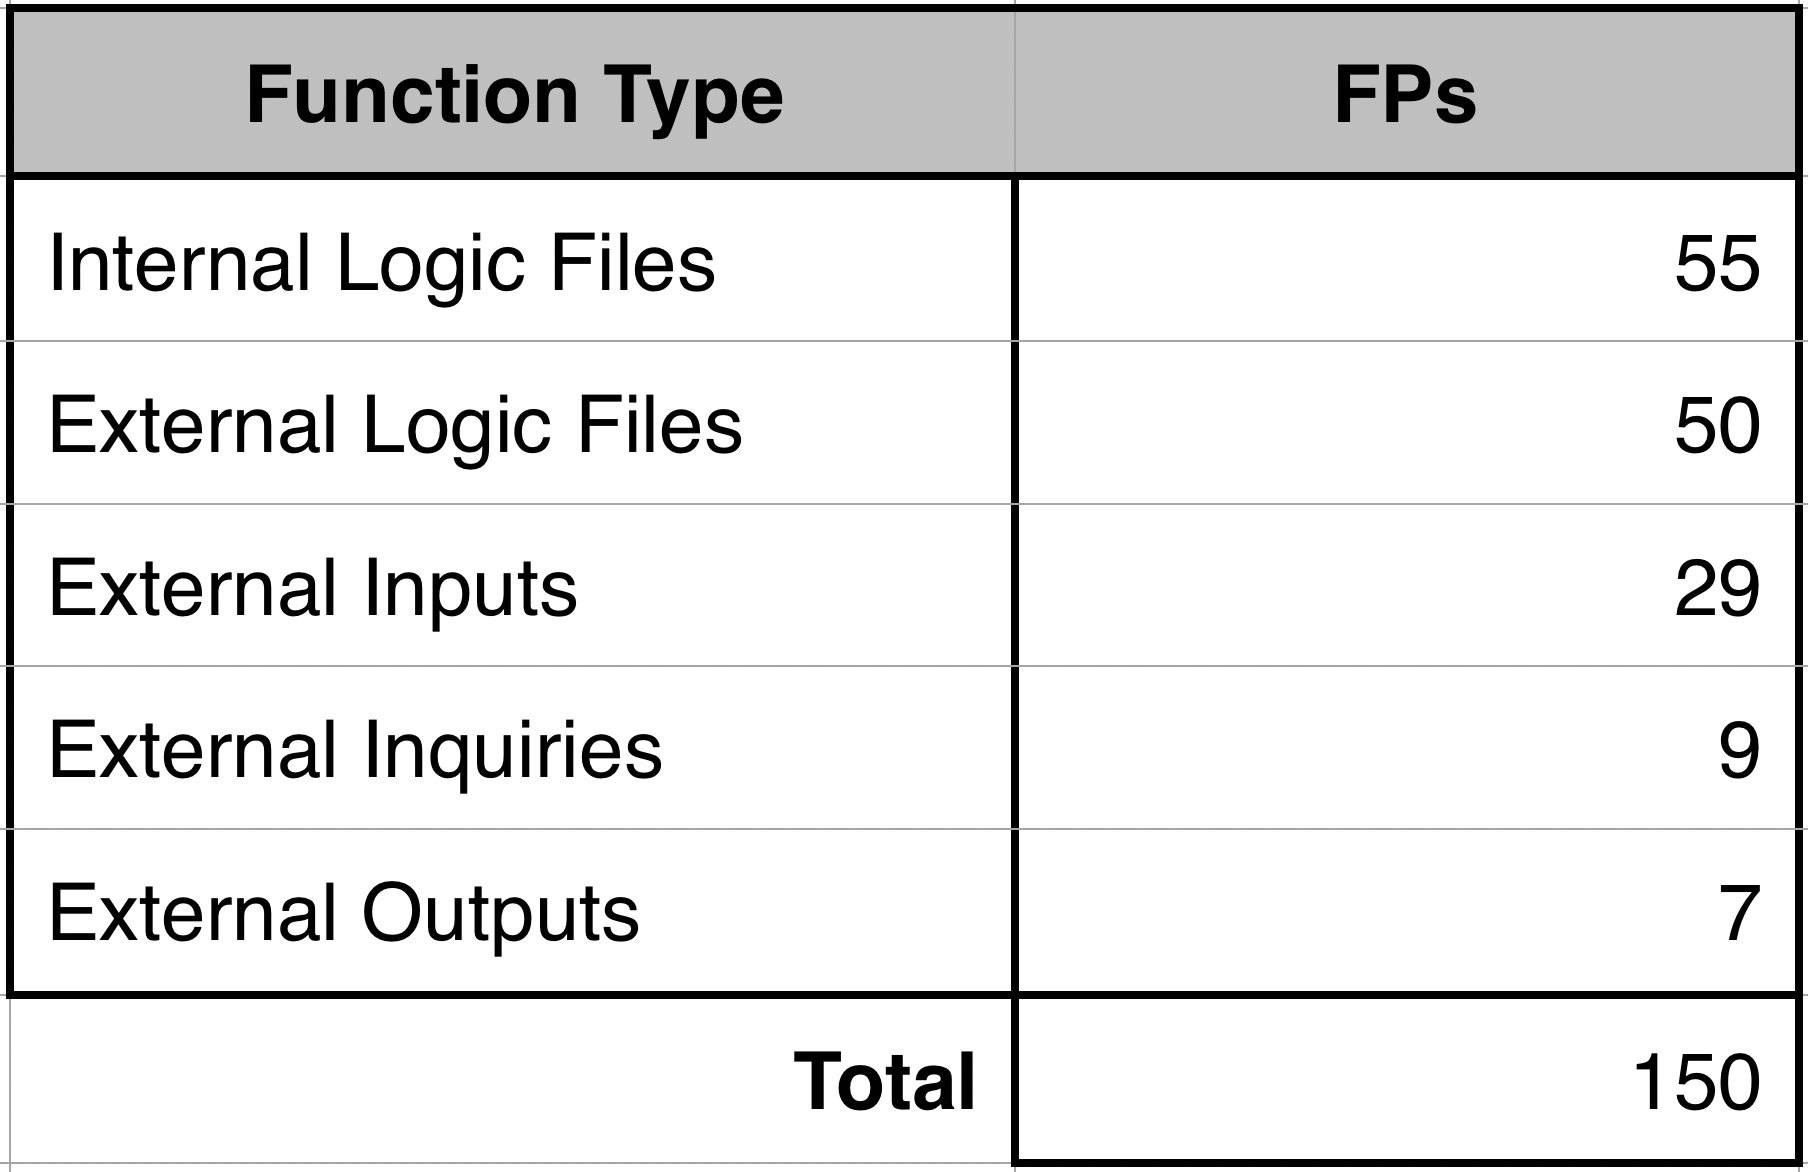
\includegraphics[scale=0.2]{Resources/overall.png}
    \caption{Overall Function Points, Resume Table}
  \end{figure}
  For the method of the function types have been defined tables (derived once more from statistical analysis) to map the number of function points
  of an application into the estimate number of lines of source code needed to implement the business logic of the considered application, 
  depending on the language used for the development.
  The figures that we found for the mapping of one function point into lines of JEE code are a lower bound of 46 and an upper bound
  of 67. This means that for each 
  function point will be needed between 46 and 67 lines of code, in order to actually implement it.
  Thus, we can comput the estimated number of lines of code for the PowerEnjoy application as:\\
    \begin{figure}[h]
  \centering
    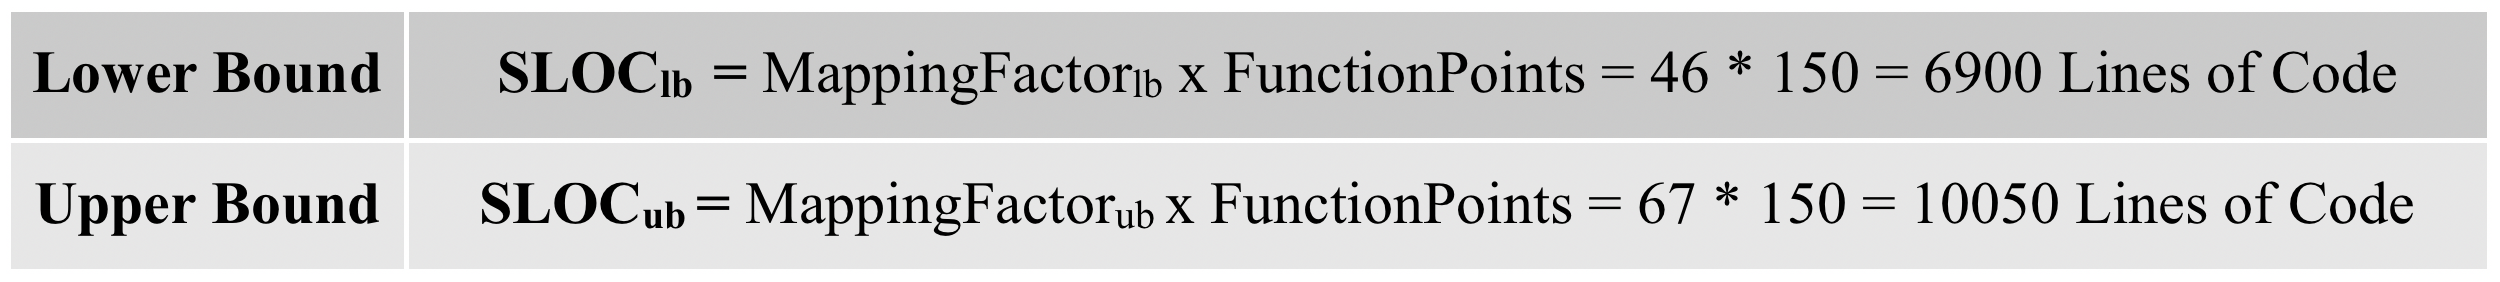
\includegraphics[scale=0.32]{Resources/sloc.png}
  \end{figure}
  \bigskip \\The estimated number of source lines of code (SLOC) varies, for this reason, in the range between 6900 and 10050.
  \subsection{Cost and Effort Estimation: COCOMO II}
  As announced in the Introduction in this section we are going to estimate the cost and effort that will be needed in order
  to successfully design and implement the application for the PowerEnjoy service. In order to do so we are going to follow the 
  COCOMO II approach.
  \FloatBarrier
  \subsubsection{Scale Drivers}
  Before listing the values for all the scale drivers, as they have been computed by the team, we attach the COCOMO II table for the scale 
  factors, extracted from the official documentation.
    \begin{figure}[h]
  \centering
    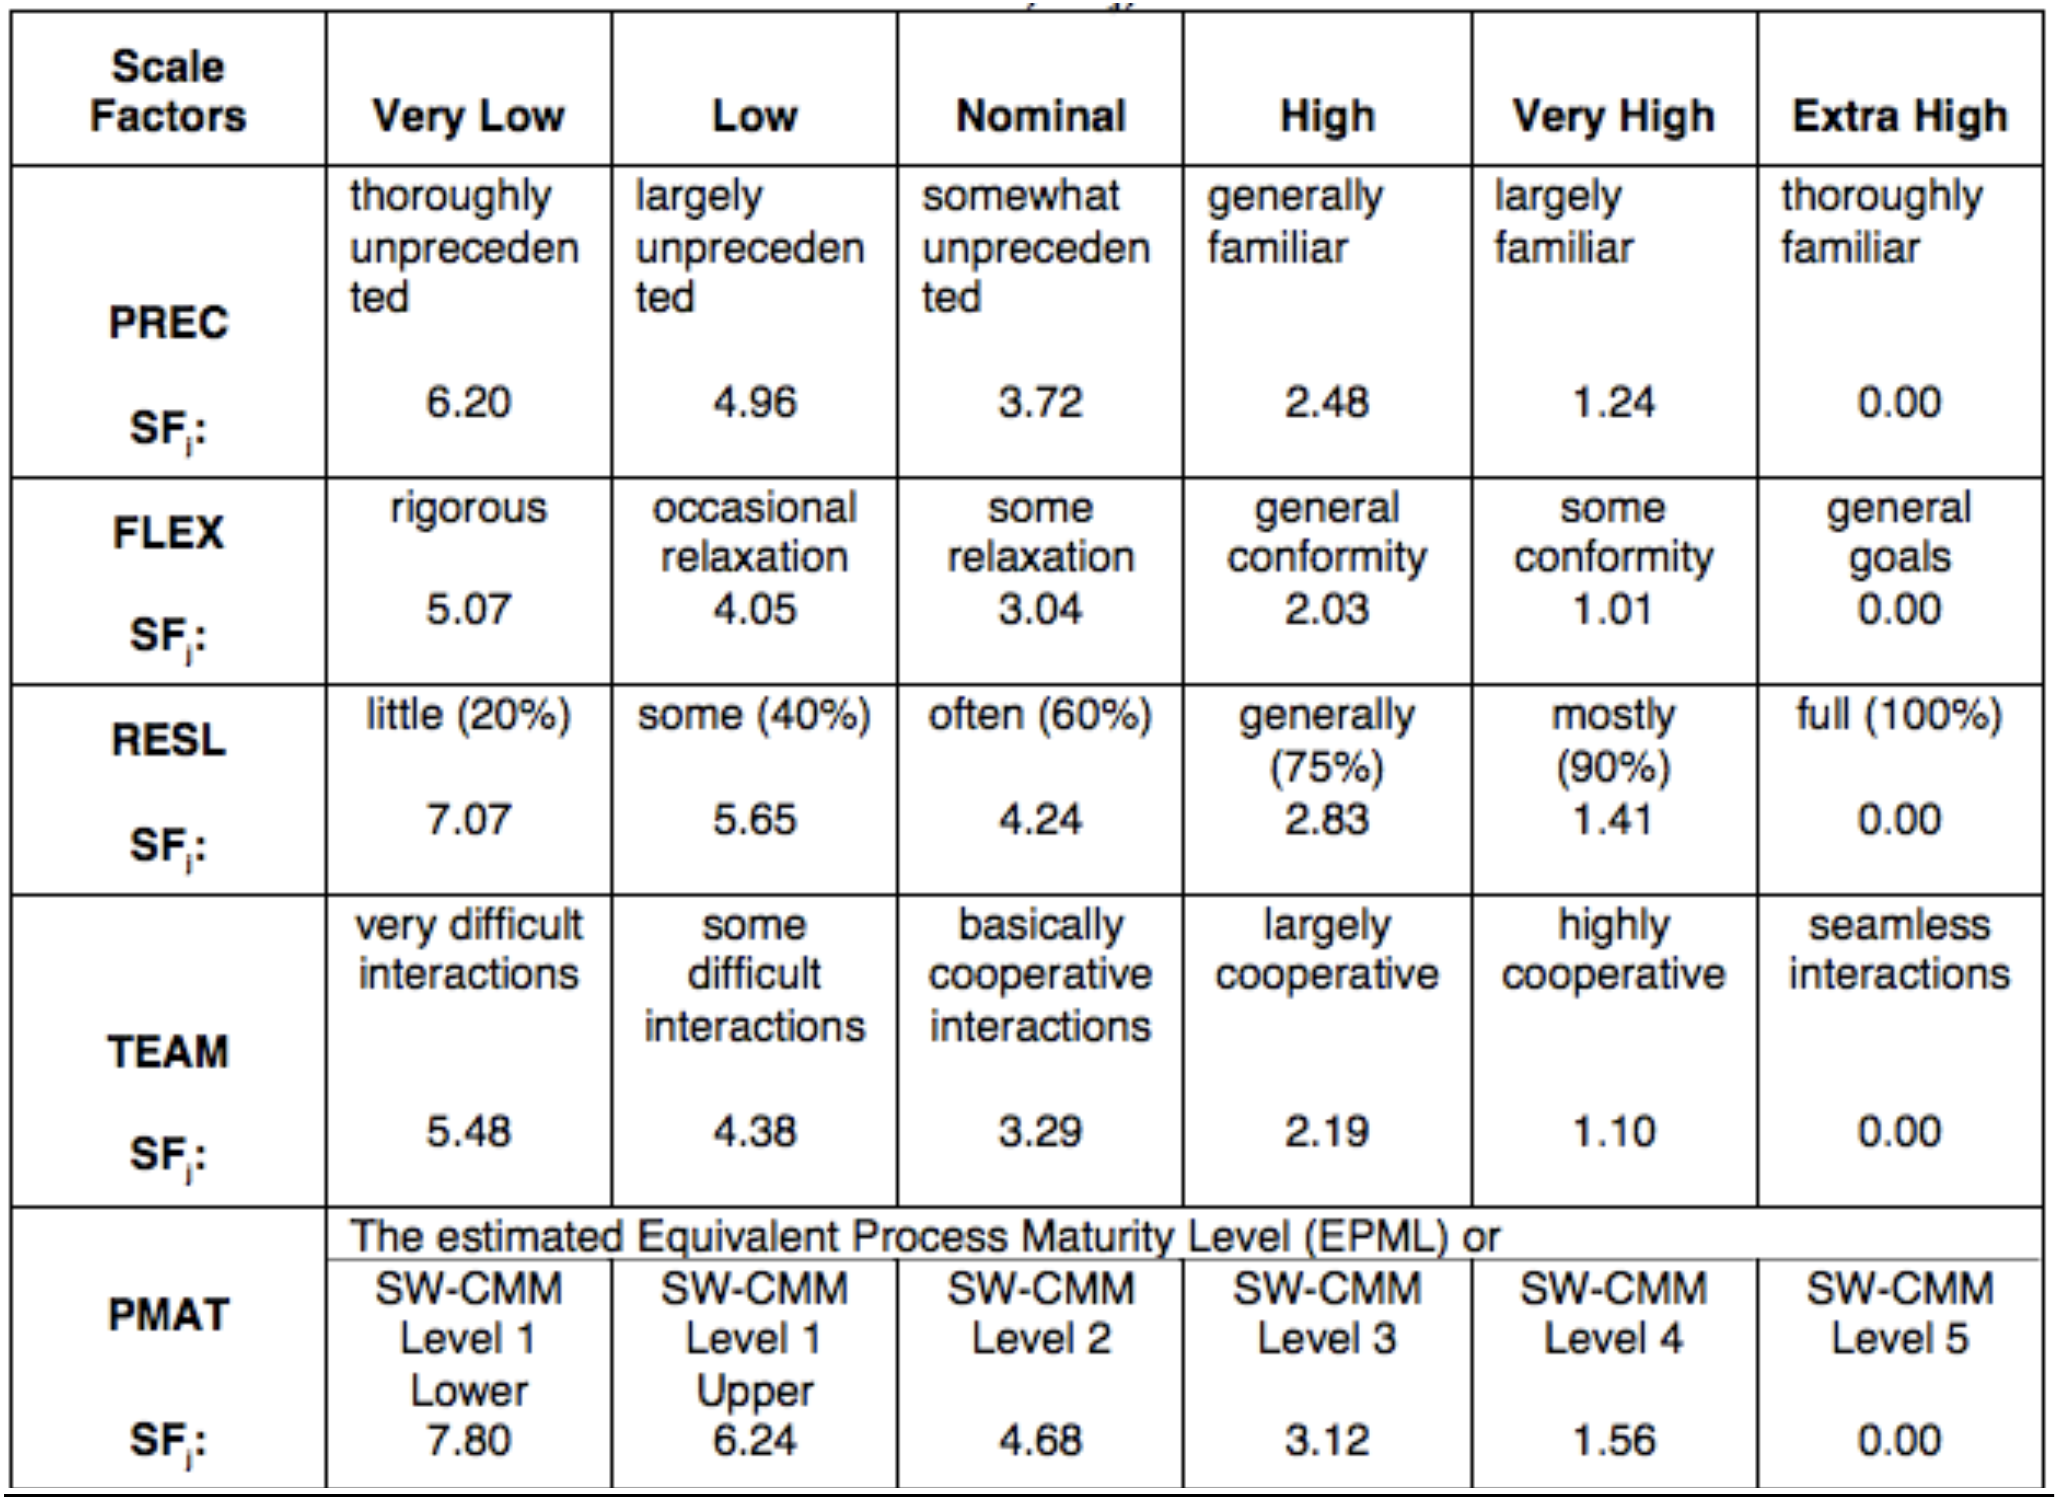
\includegraphics[scale=0.32]{Resources/cocomo/cocomo_ge.png}
  \end{figure}
  \FloatBarrier
  Here it follows a brief description for each of the scale drivers that have been analyzed:
   \begin{description}
    \item[$\bullet$] \textbf{Precedentedness:} Since the components of our team have worked on other similar projects together although we can’t consider ourselves experts in this kind of project, we will give a \textbf{nominal} precedentedness value.
    \item[$\bullet$] \textbf{Development Flexibility:} Our project has been scheduled and guided by a set of deadlines and requirements provided by software engineering 2 course, but its also fair to state that the implementation and description of the system structure has been build by us nearly from scratch, meaning that we’ve been able to make our assumptions and choose the technologies to use. For this reason this section will have a value of \textbf{low}.
    \item[$\bullet$] \textbf{Risk Resolution:} The percent of development schedule devoted to establish an architecture is high, moreover, the risk analysis we performed pretends to treat nearly all sections of our work.  Our team of qualified software architects has also been using specific support tools to reduce the amount of uncertainty in key architecture drivers. Hence this value will be set to \textbf{very high}. 
    \item[$\bullet$] \textbf{Team Cohesion:} Our team members know each other very well and have experience working together. This coefficient is set to \textbf{extra high}.
    \item[$\bullet$] \textbf{Process Maturity:} Although our project accomplishes all required goals, we have seen that there’s a part of our system concerning the database distribution architecture in internal and external systems that should be reviewed to decide which option is optimal. For this reason we will give this section a \textbf{level 4}.
  \end{description}
      \begin{figure}[h]
  \centering
    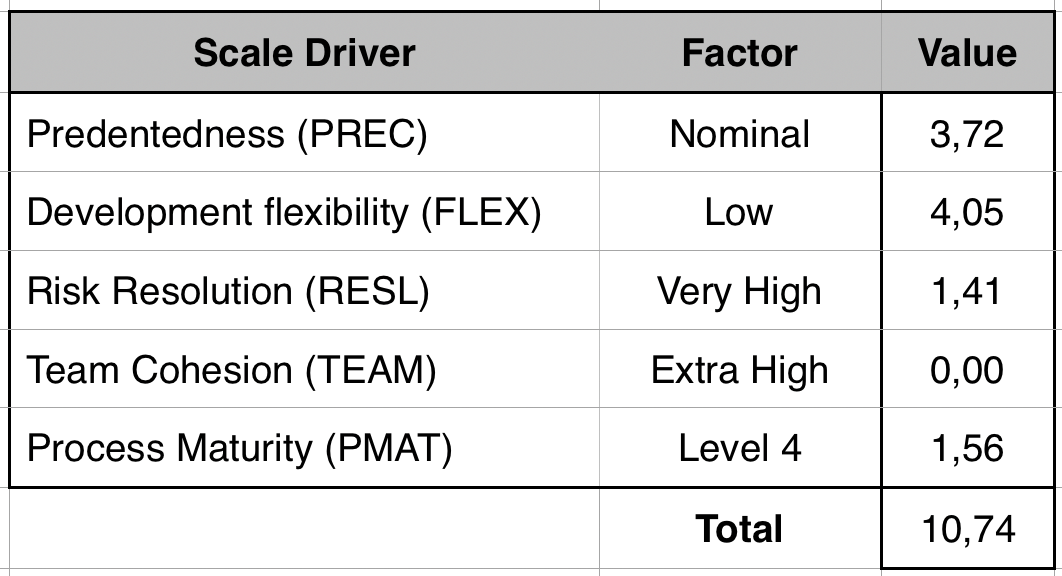
\includegraphics[scale=0.32]{Resources/cocomo/resume1.png}
  \end{figure}
  \FloatBarrier
  \subsubsection{Cost Drivers (post-Architecture)}
  \begin{description}
  \item[$\bullet$] \textbf{Required Software Reliability:} Our system has the bank details of users and manages fees and billings, for this reason it requires a \textbf{high} reliability.
        \begin{figure}[h]
  \centering
    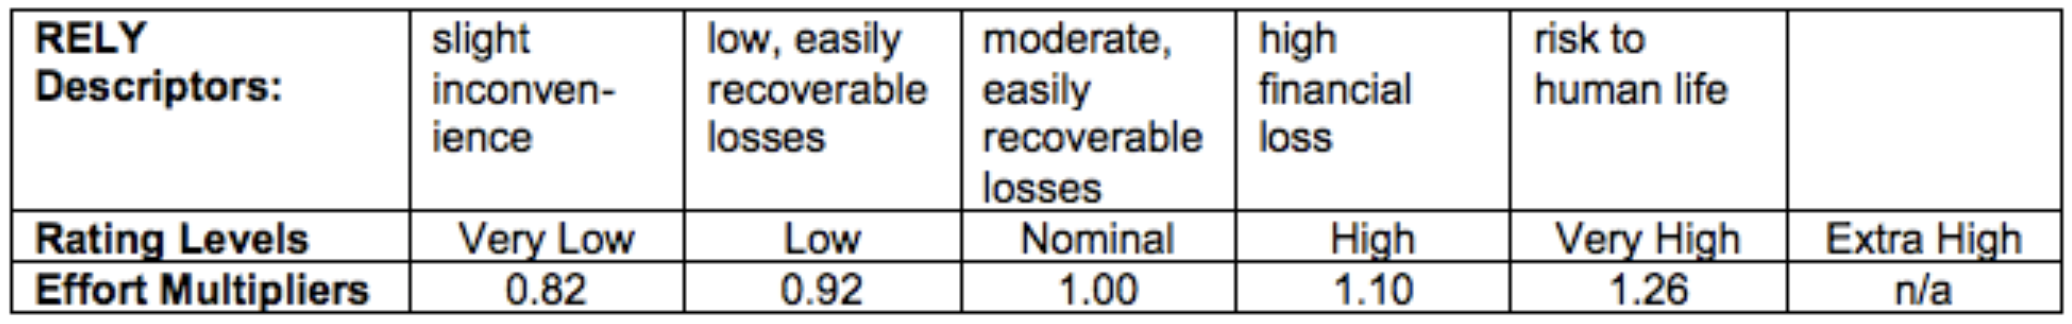
\includegraphics[scale=0.32]{Resources/cocomo/rely.png}
  \end{figure}
  \item[$\bullet$] \textbf{Database Size:}Database size: Our estimations reach the 3 GB of data for our internal database.  Hence the DATA coefficient is \textbf{very high} given a value of 8700 as SLOC.
          \begin{figure}[h]
  \centering
    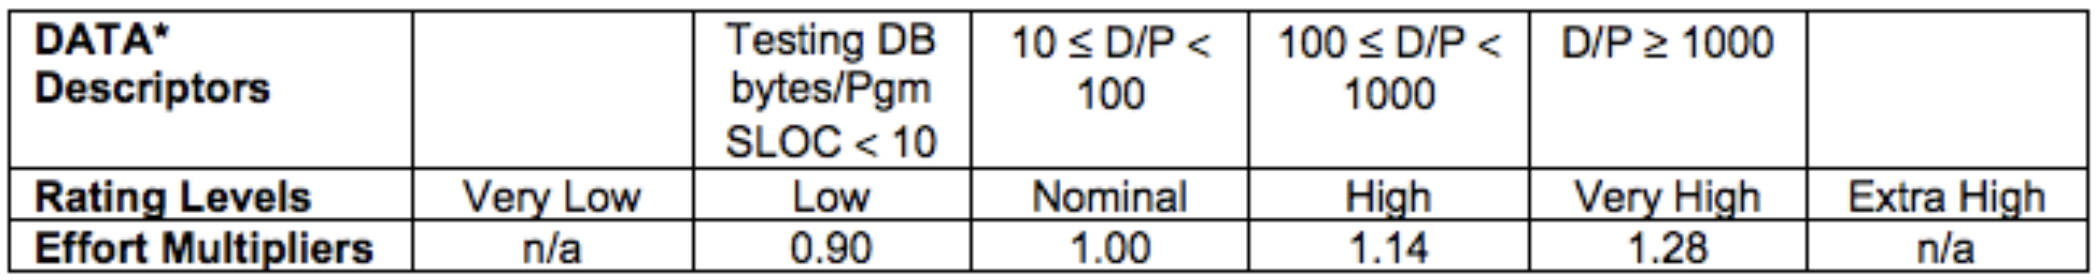
\includegraphics[scale=0.32]{Resources/cocomo/data.png}
  \end{figure}\FloatBarrier
  \item[$\bullet$] \textbf{Product Complexity:} 
     \begin{description}
    \item[$\bullet$] \textbf{Control Operations: } The operations carried out by the whole system could reach a high complexity level, but since we made the assumption that most of our operations are handled by the existing system we will set this section to a \textbf{nominal} value.
    \item[$\bullet$] \textbf{Computational Operations: } \textbf{nominal}
    \item[$\bullet$] \textbf{Device Dependent Operations: } \textbf{nominal}
    \item[$\bullet$] \textbf{Data Management Operations: } Our application will use simple triggers in its database. And since the database of the external and the internal system is not the same, they will also need some kind of synchronization. This value is set to \textbf{very high}.
    \item[$\bullet$] \textbf{User Interface Management Operations: } This value is set to \textbf{high} because the application will use extensions such as google maps to represent the cars apart from possibly developing a widget set for the DBMS. 
    \item Computing the average of the previous coefficients, we will give a \textbf{nominal} value to Product complexity.  
  \end{description}
\item[$\bullet$] \textbf{Required Reusability:} The required reusability is \textbf{high} because we are extending and reusing parts of an already made product, and it is fairly reasonable to expect the usage of the application in a future. 
          \begin{figure}[!h]
  \centering
    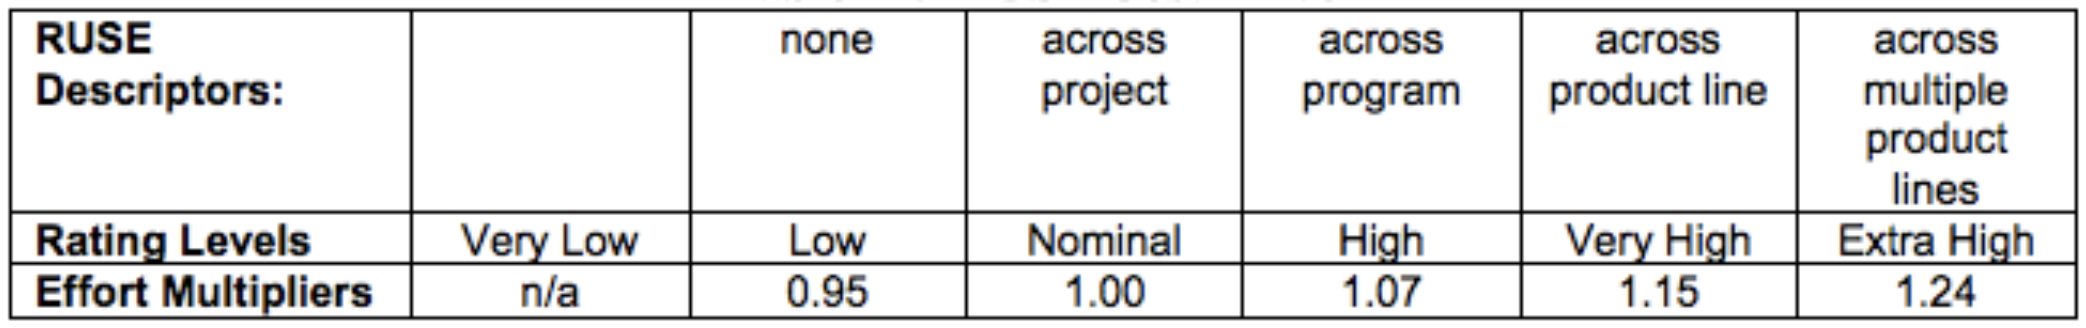
\includegraphics[scale=0.32]{Resources/cocomo/ruse.png}
  \end{figure}\FloatBarrier\item[$\bullet$] \textbf{Documentation Match to life Cycle Needs:} From our point of view, it is right sized to life-cycle needs, thus we assign a rate of \textbf{nominal}.
          \begin{figure}[!h]
  \centering
    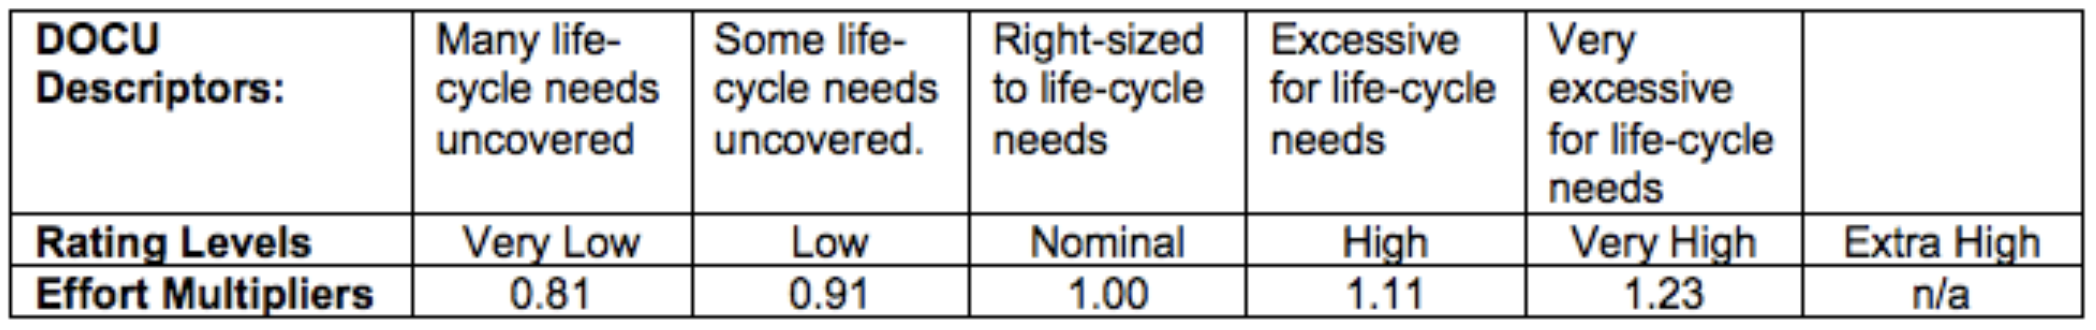
\includegraphics[scale=0.32]{Resources/cocomo/docu.png}
  \end{figure}\FloatBarrier
  \item[$\bullet$] \textbf{Execution Time Constraint:} We will set this value to \textbf{nominal} because although the software is complex, the time dedicated to its operations is relatively small.
          \begin{figure}[!h]
  \centering
    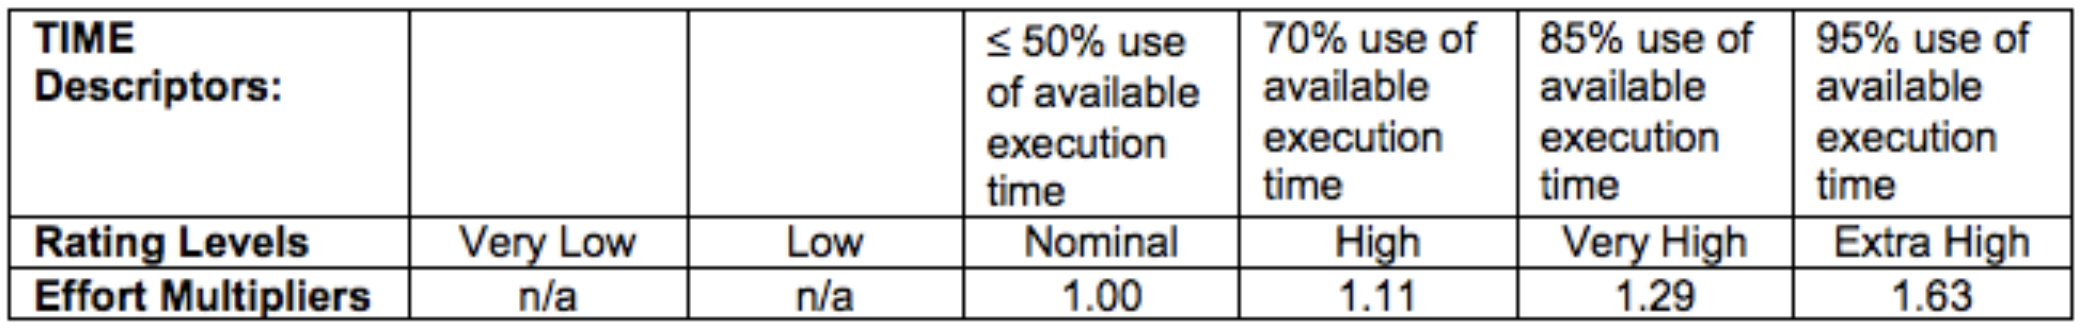
\includegraphics[scale=0.32]{Resources/cocomo/time.png}
  \end{figure}\FloatBarrier
  \item[$\bullet$] \textbf{Main Storage Constraint:} Our system doesn’t require significant amount of storage, this value is set to \textbf{nominal}.
          \begin{figure}[!h]
  \centering
    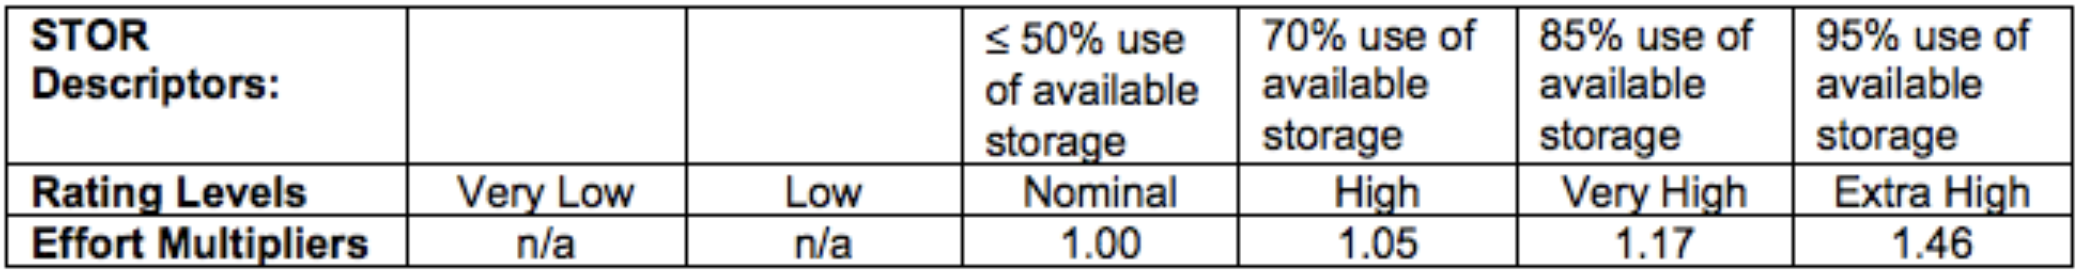
\includegraphics[scale=0.32]{Resources/cocomo/stor.png}
  \end{figure}\FloatBarrier
  \item[$\bullet$] \textbf{Platform Volatility:} Keeping in mind that we are developing a software including a DBMS, that depends on two other external systems, this value should be between nominal and high, so we will set it to \textbf{high}.
          \begin{figure}[!h]
  \centering
    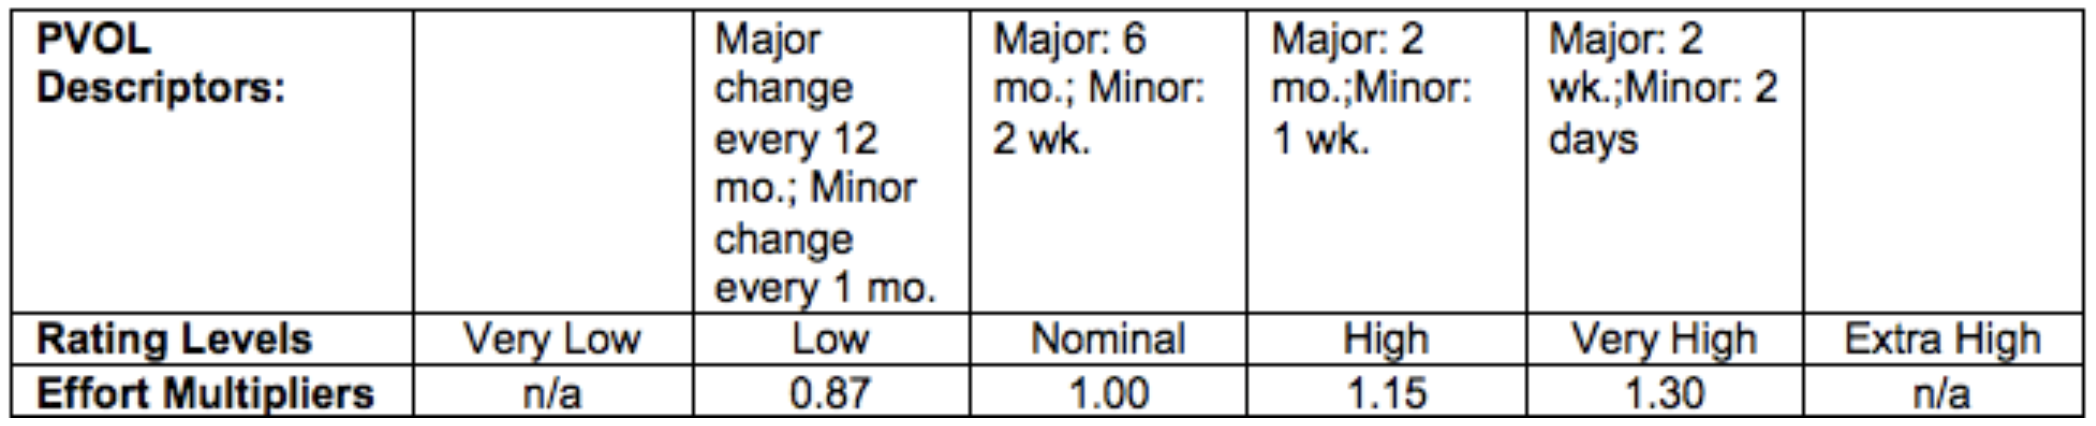
\includegraphics[scale=0.32]{Resources/cocomo/pvol.png}
  \end{figure}
  \item[$\bullet$] \textbf{Analyst Capability:} The requirements and design features have been built following high-level procedures and references by the team. 
          \begin{figure}[!h]
  \centering
    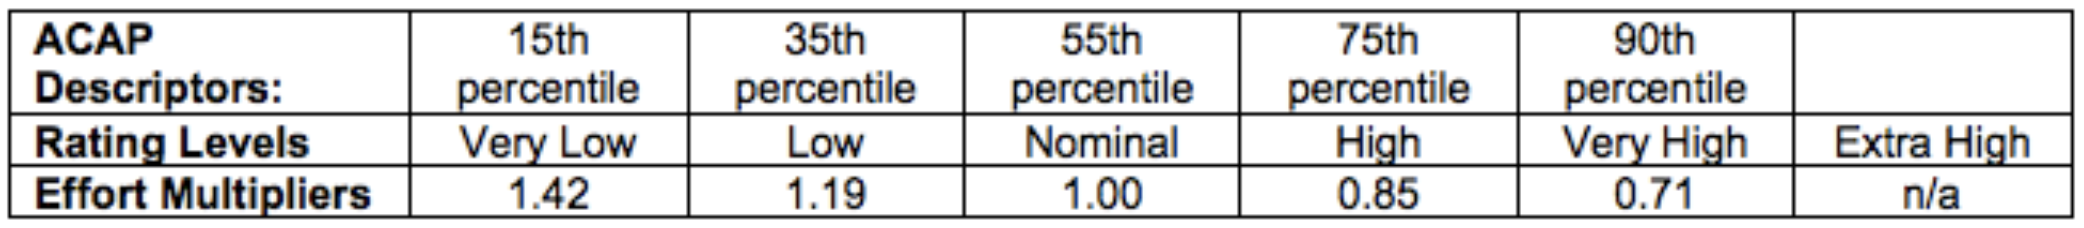
\includegraphics[scale=0.32]{Resources/cocomo/acap.png}
  \end{figure}\FloatBarrier
  \item[$\bullet$] \textbf{Programmer Capability:} The team programming skills should be considered as \textbf{high}.
          \begin{figure}[!h]
  \centering
    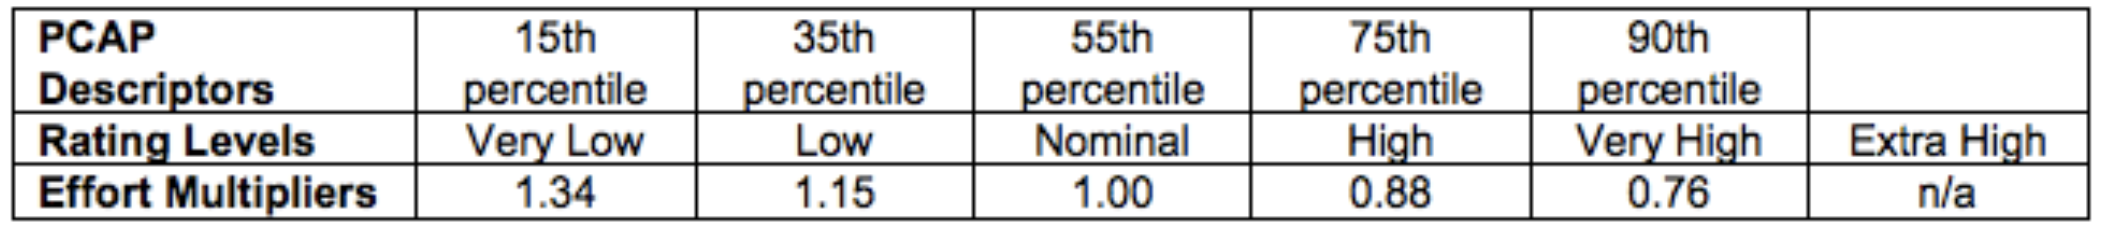
\includegraphics[scale=0.32]{Resources/cocomo/pcap.png}
  \end{figure}\FloatBarrier
  \item[$\bullet$] \textbf{Personnel Continuity:} The value is set to \textbf{very low} because all our team will be replaced.
          \begin{figure}[!h]
  \centering
    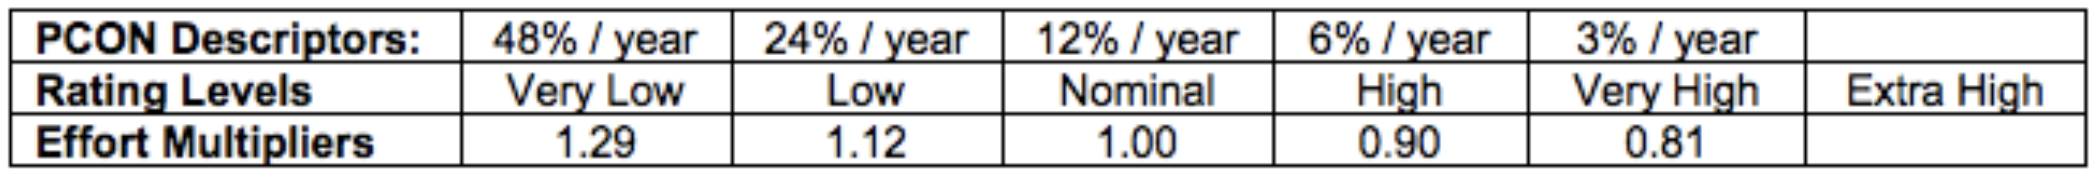
\includegraphics[scale=0.17]{Resources/cocomo/pcon.png}
  \end{figure}\FloatBarrier
  \item[$\bullet$] \textbf{Applications Experience:} The value is set to \textbf{low} because the team has more than 6 months of experience on the majority of the project sections, but not all of them.
          \begin{figure}[!h]
  \centering
    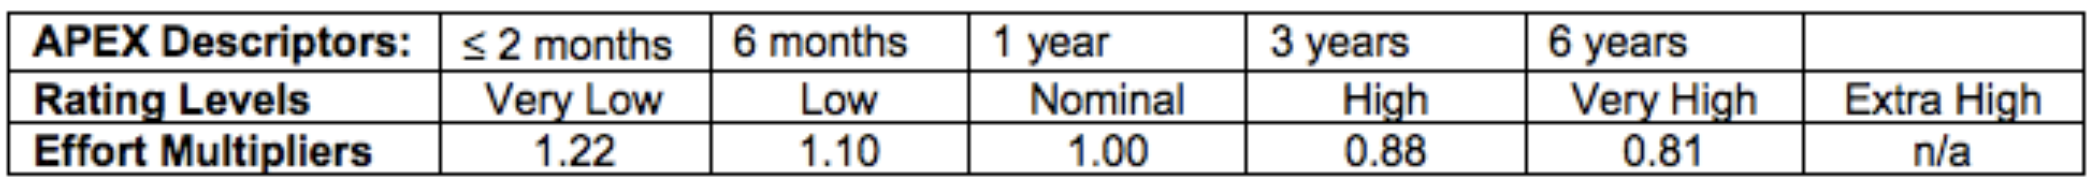
\includegraphics[scale=0.17]{Resources/cocomo/apex.png}
  \end{figure}\FloatBarrier
  \item[$\bullet$] \textbf{Platform Experience:} The experience of our team with the used platforms is to be considered \textbf{nominal}.
          \begin{figure}[!h]
  \centering
    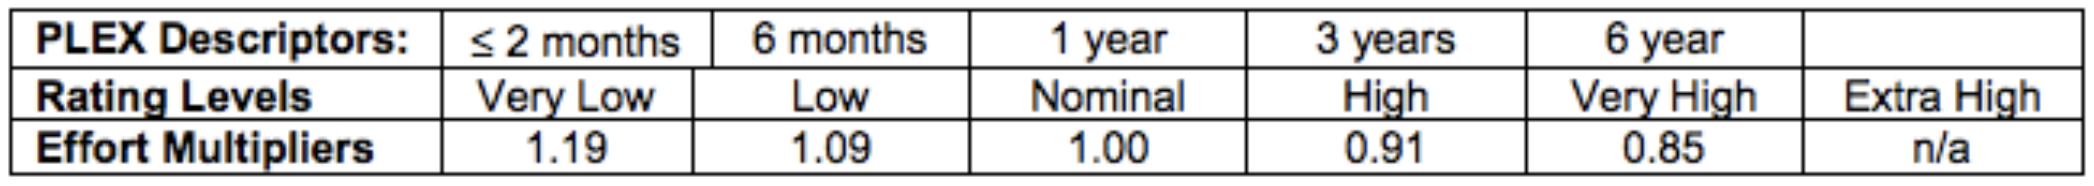
\includegraphics[scale=0.17]{Resources/cocomo/plex.png}
  \end{figure}\FloatBarrier
  \item[$\bullet$] \textbf{Language and Tool Experience:} This value is set to \textbf{nominal} for our team.
          \begin{figure}[!h]
  \centering
    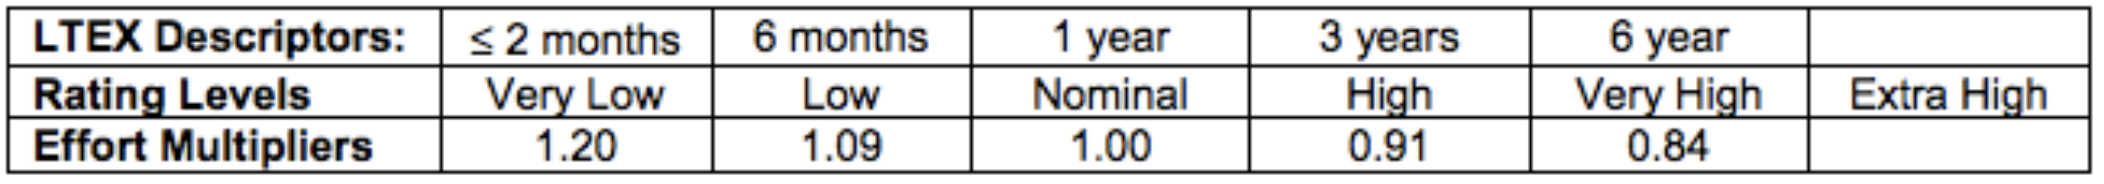
\includegraphics[scale=0.17]{Resources/cocomo/ltex.png}
  \end{figure}\FloatBarrier
  \item[$\bullet$] \textbf{Use of Software Tools:} The extension and variety of the system demands a \textbf{high level} in this section.
          \begin{figure}[!h]
  \centering
    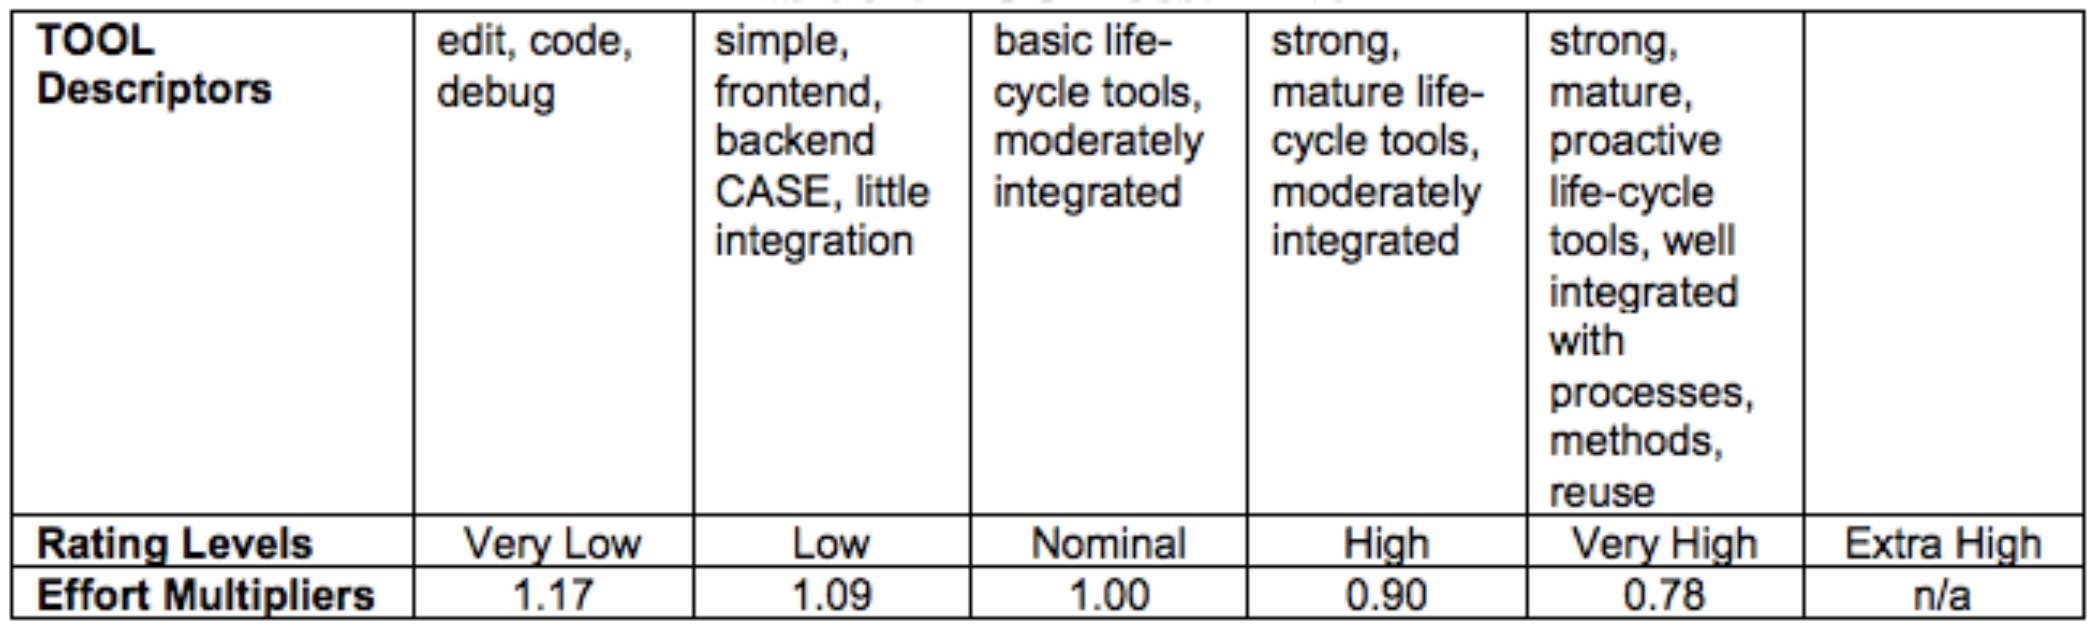
\includegraphics[scale=0.32]{Resources/cocomo/tool.png}
  \end{figure}\FloatBarrier
  \item[$\bullet$] \textbf{Multisite Development:} The site collocation should be the same city, at least for the part of system that we are developing, and the communication support correspond to a \textbf{high} level as well.
          \begin{figure}[!h]
  \centering
    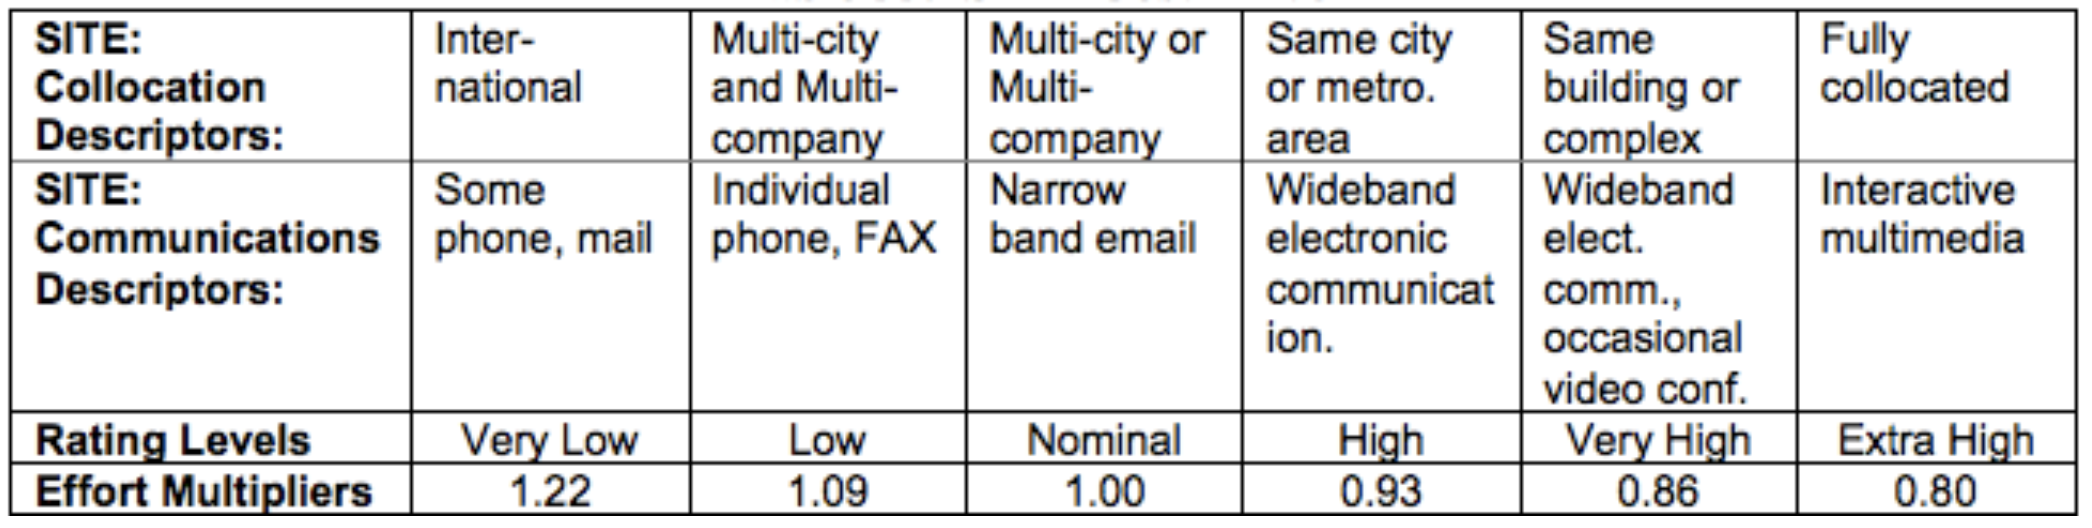
\includegraphics[scale=0.32]{Resources/cocomo/site.png}
  \end{figure}\FloatBarrier
  \item[$\bullet$] \textbf{Required Development Schedule:} Although we have spent a significant amount of time planning and designing the project, we also expect to dedicate a large amount of time to development, for this reason we give it a value of \textbf{nominal}.
          \begin{figure}[!h]
  \centering
    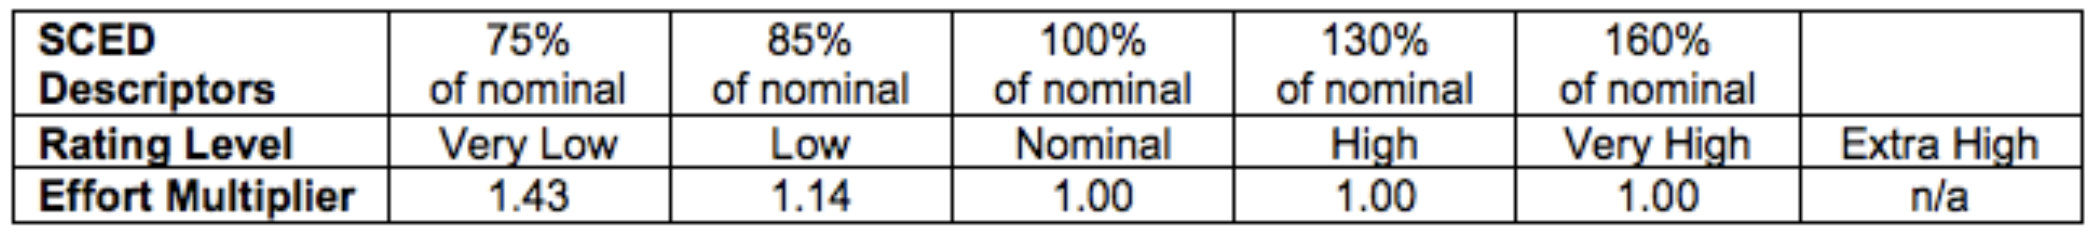
\includegraphics[scale=0.32]{Resources/cocomo/sced.png}
  \end{figure}\FloatBarrier

\end{description}
    \bigskip And finally we attach the resume table of the cost driver evaluation:
        \begin{figure}[!h]
  \centering

    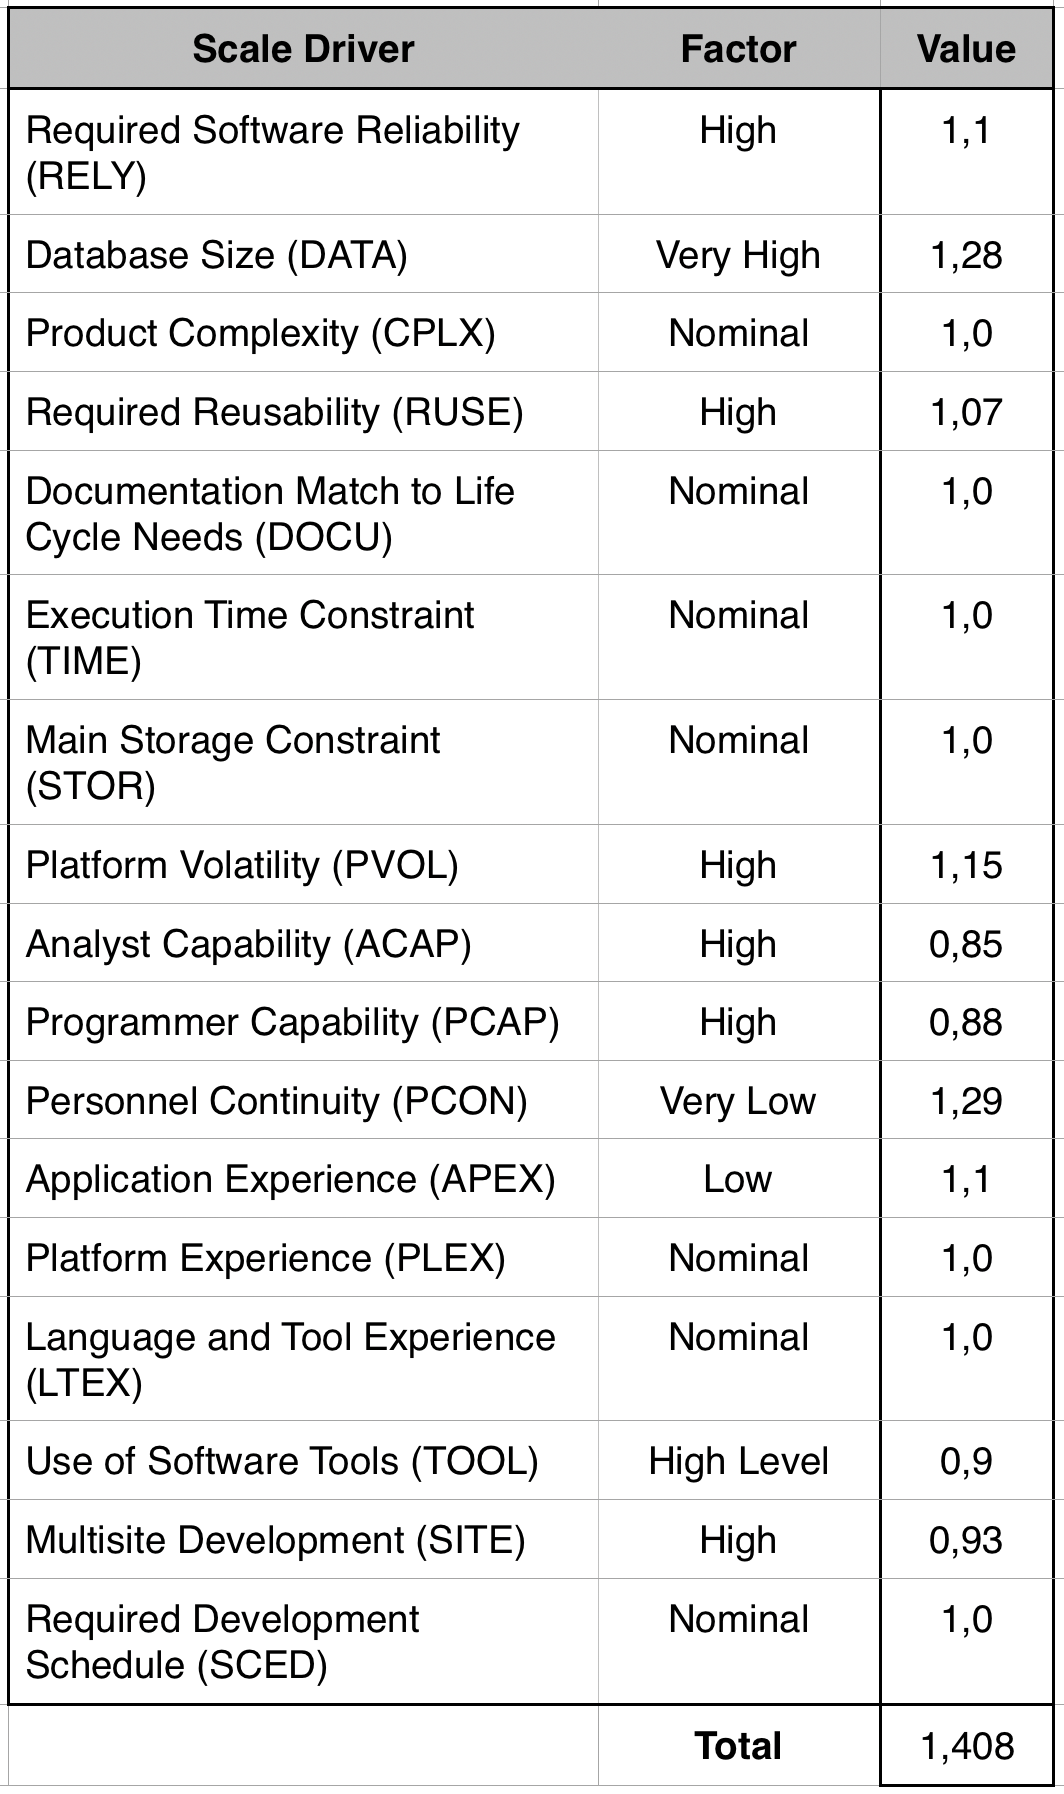
\includegraphics[scale=0.40]{Resources/cocomo/resume2.png}
  \end{figure}\FloatBarrier
  \subsubsection{Effort Equation}
  After the above reported evaluations is possible to use the effort estimation in Person-Months (PM):
  \begin{center}
    Effort = A * EAF * KSLOC\textsuperscript{E}\\\bigskip
    where:\\\bigskip
    A = 2.94 (for COCOMO II)\\\bigskip
    EAF = [product of all cost drivers] = 1.5391 \\\bigskip
    E = [exponent derived from the scale drivers] =\\
    = B + 0.01 * $\sum_{i}{SF_i}$ = B + 0.01 * 10.74 = 1.0174\\\bigskip
    in which B is equal to 0.91 for COCOMO II
  \end{center}
  Thanks to the above computed parameters we can compute the effort estimation respectively for
  the lower and upper bound given for the SLOCs:
    \begin{center}
    Effort_{lb} = A * EAF * KSLOC_{lb}\textsuperscript{E} = 2.94 * 1.5391 * 6.9\textsuperscript{1.0174} = 32.29 PM\\\bigskip
    Effort_{ub} = A * EAF * KSLOC_{ub}\textsuperscript{E} = 2.94 * 1.5391 * 10.05\textsuperscript{1.0174} = 47.34 PM
    \\\bigskip
  \end{center}
  And a consequent Schedule estimation given by the following formula (again both for the lower and the upper bound):
  \begin{center}
    Duration = 3.67 * Effort\textsuperscript{F}\\\bigskip
    where:\\\bigskip
    F = 0.28 + 0.2 * (E-B) = 0.28 + 0.2 * 0.1074 = 0.3014
    \\\bigskip
  \end{center}
  And from that we can compute the upper and lower bound for the estimated duration of the project:
  \begin{center}
    Duration_{lb} = 3.67 * Effort_{lb}\textsuperscript{F} = 3.67 * 32.29\textsuperscript{0.3014} = 10.45 Months\\\bigskip
    Duration_{ub} = 3.67 * Effort_{ub}\textsuperscript{F} = 3.67 * 47.34\textsuperscript{0.3014} = 11.73 Months\\\bigskip

  \end{center}
  In conclusion we can assume that the effort necessary to carry out the project is included in the interval between 32.29 and 47.34 person 
  per month and thus, the estimated duration of the project varies between 10.45 and 11.74 months.
  \clearpage\section{Schedule} In the following section we are going to provide an high-level project schedule.\\ Although the project is
  made for didactic purpose and no development is going to take place, we are going to include in the following schedule
  the steps that we will not actually do.\\ Since the dimension of the schedule was quite big it has been splitted in two parts: the first 
  represents the activities actually performed by the team. The second instead is the part of the schedule concerning the future development 
  of the PowerEnjoy application.\\\bigskip
            \begin{figure}[!h]
  \centering
    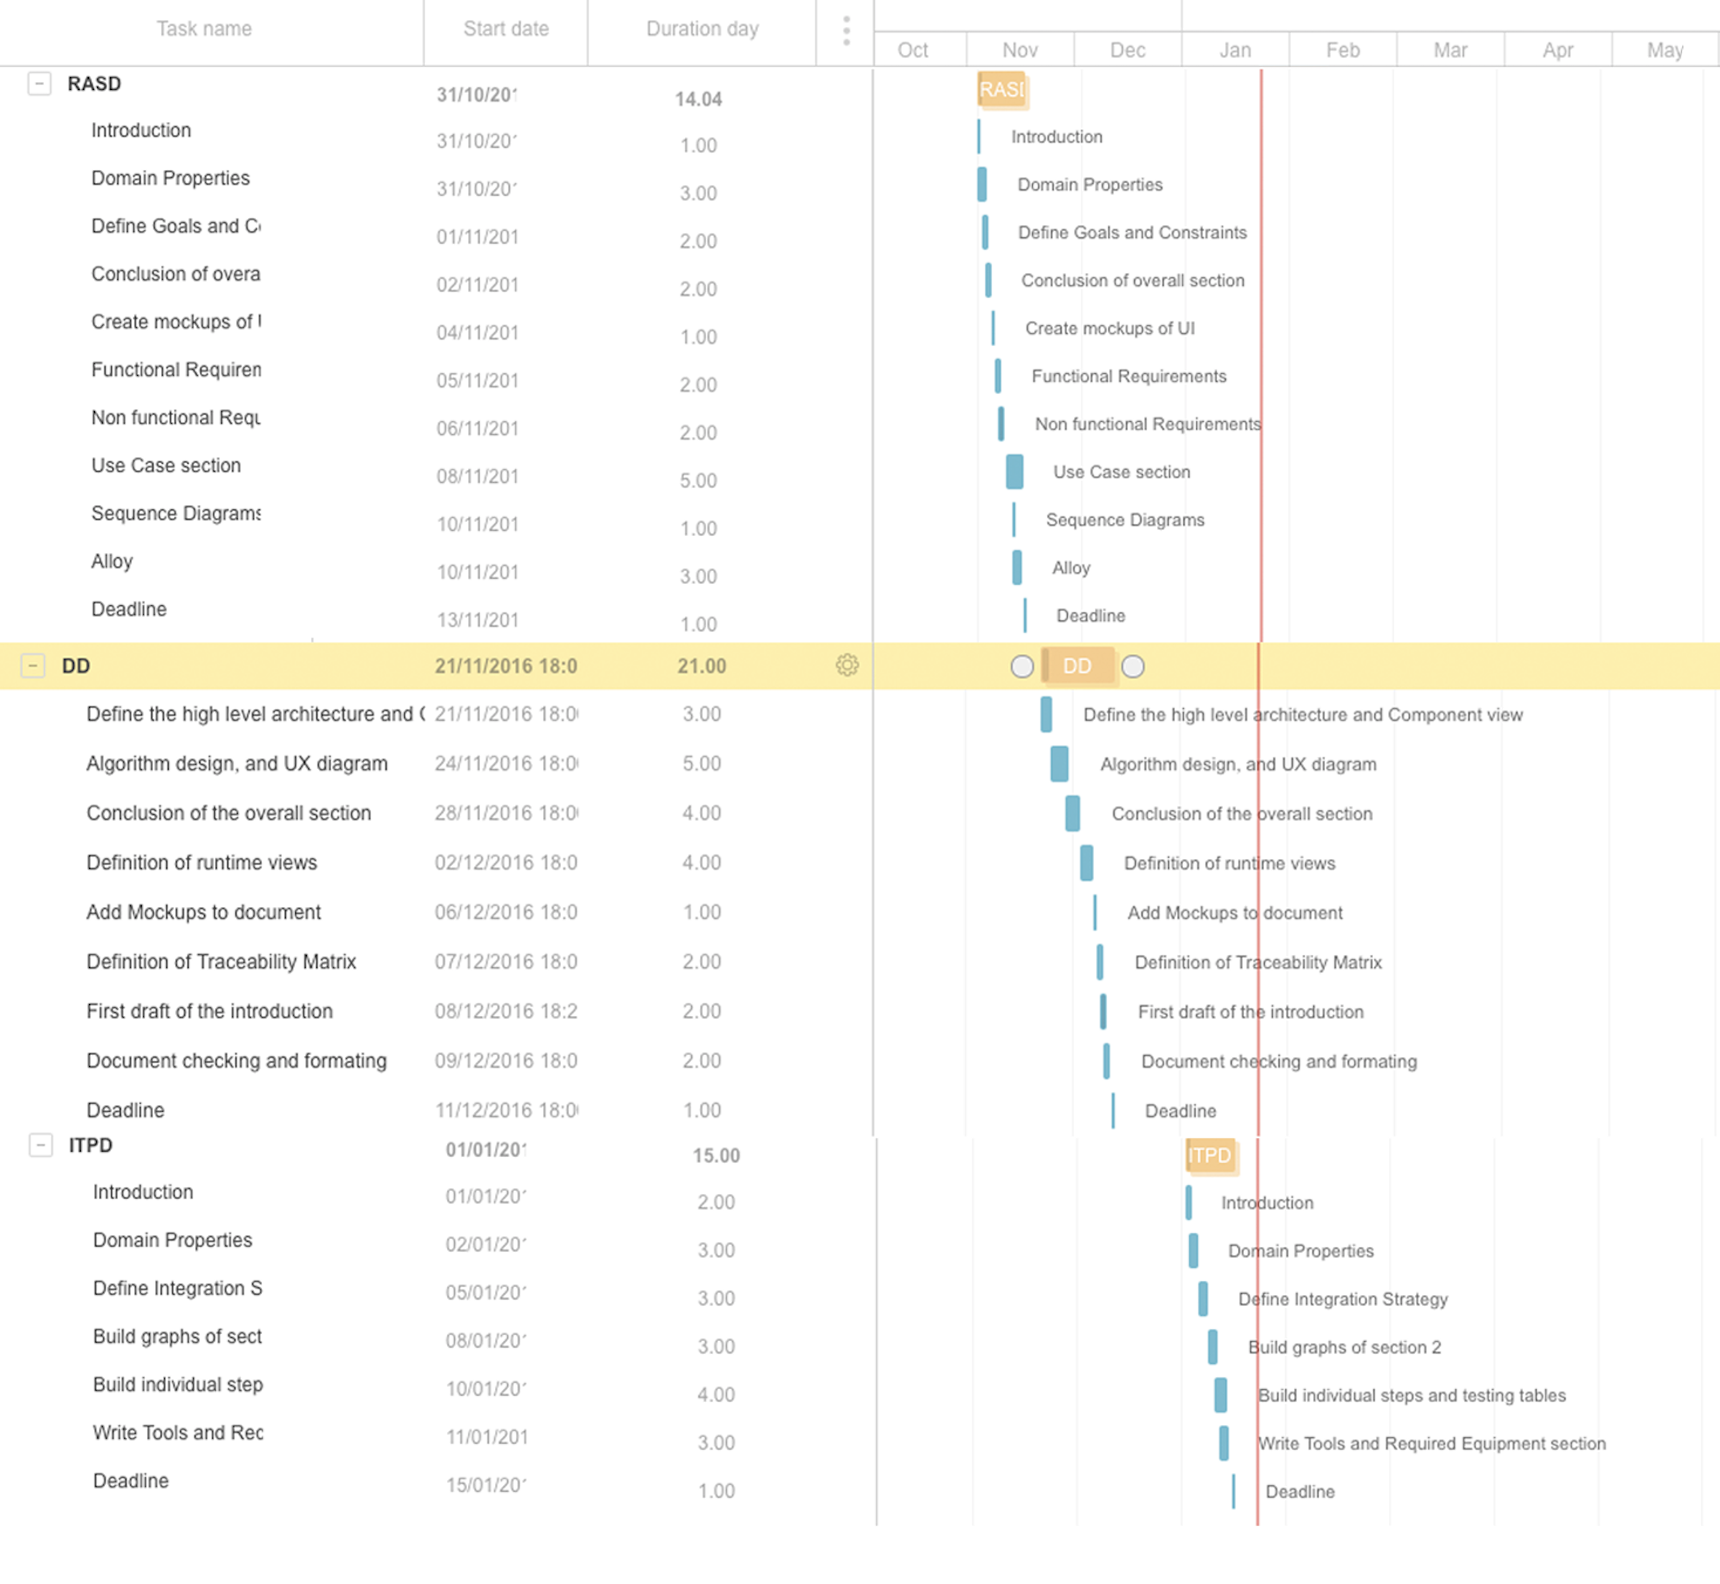
\includegraphics[scale=0.50]{Resources/gant1.png}
  \end{figure}\FloatBarrier
  \begin{figure}[!h]
  \centering
    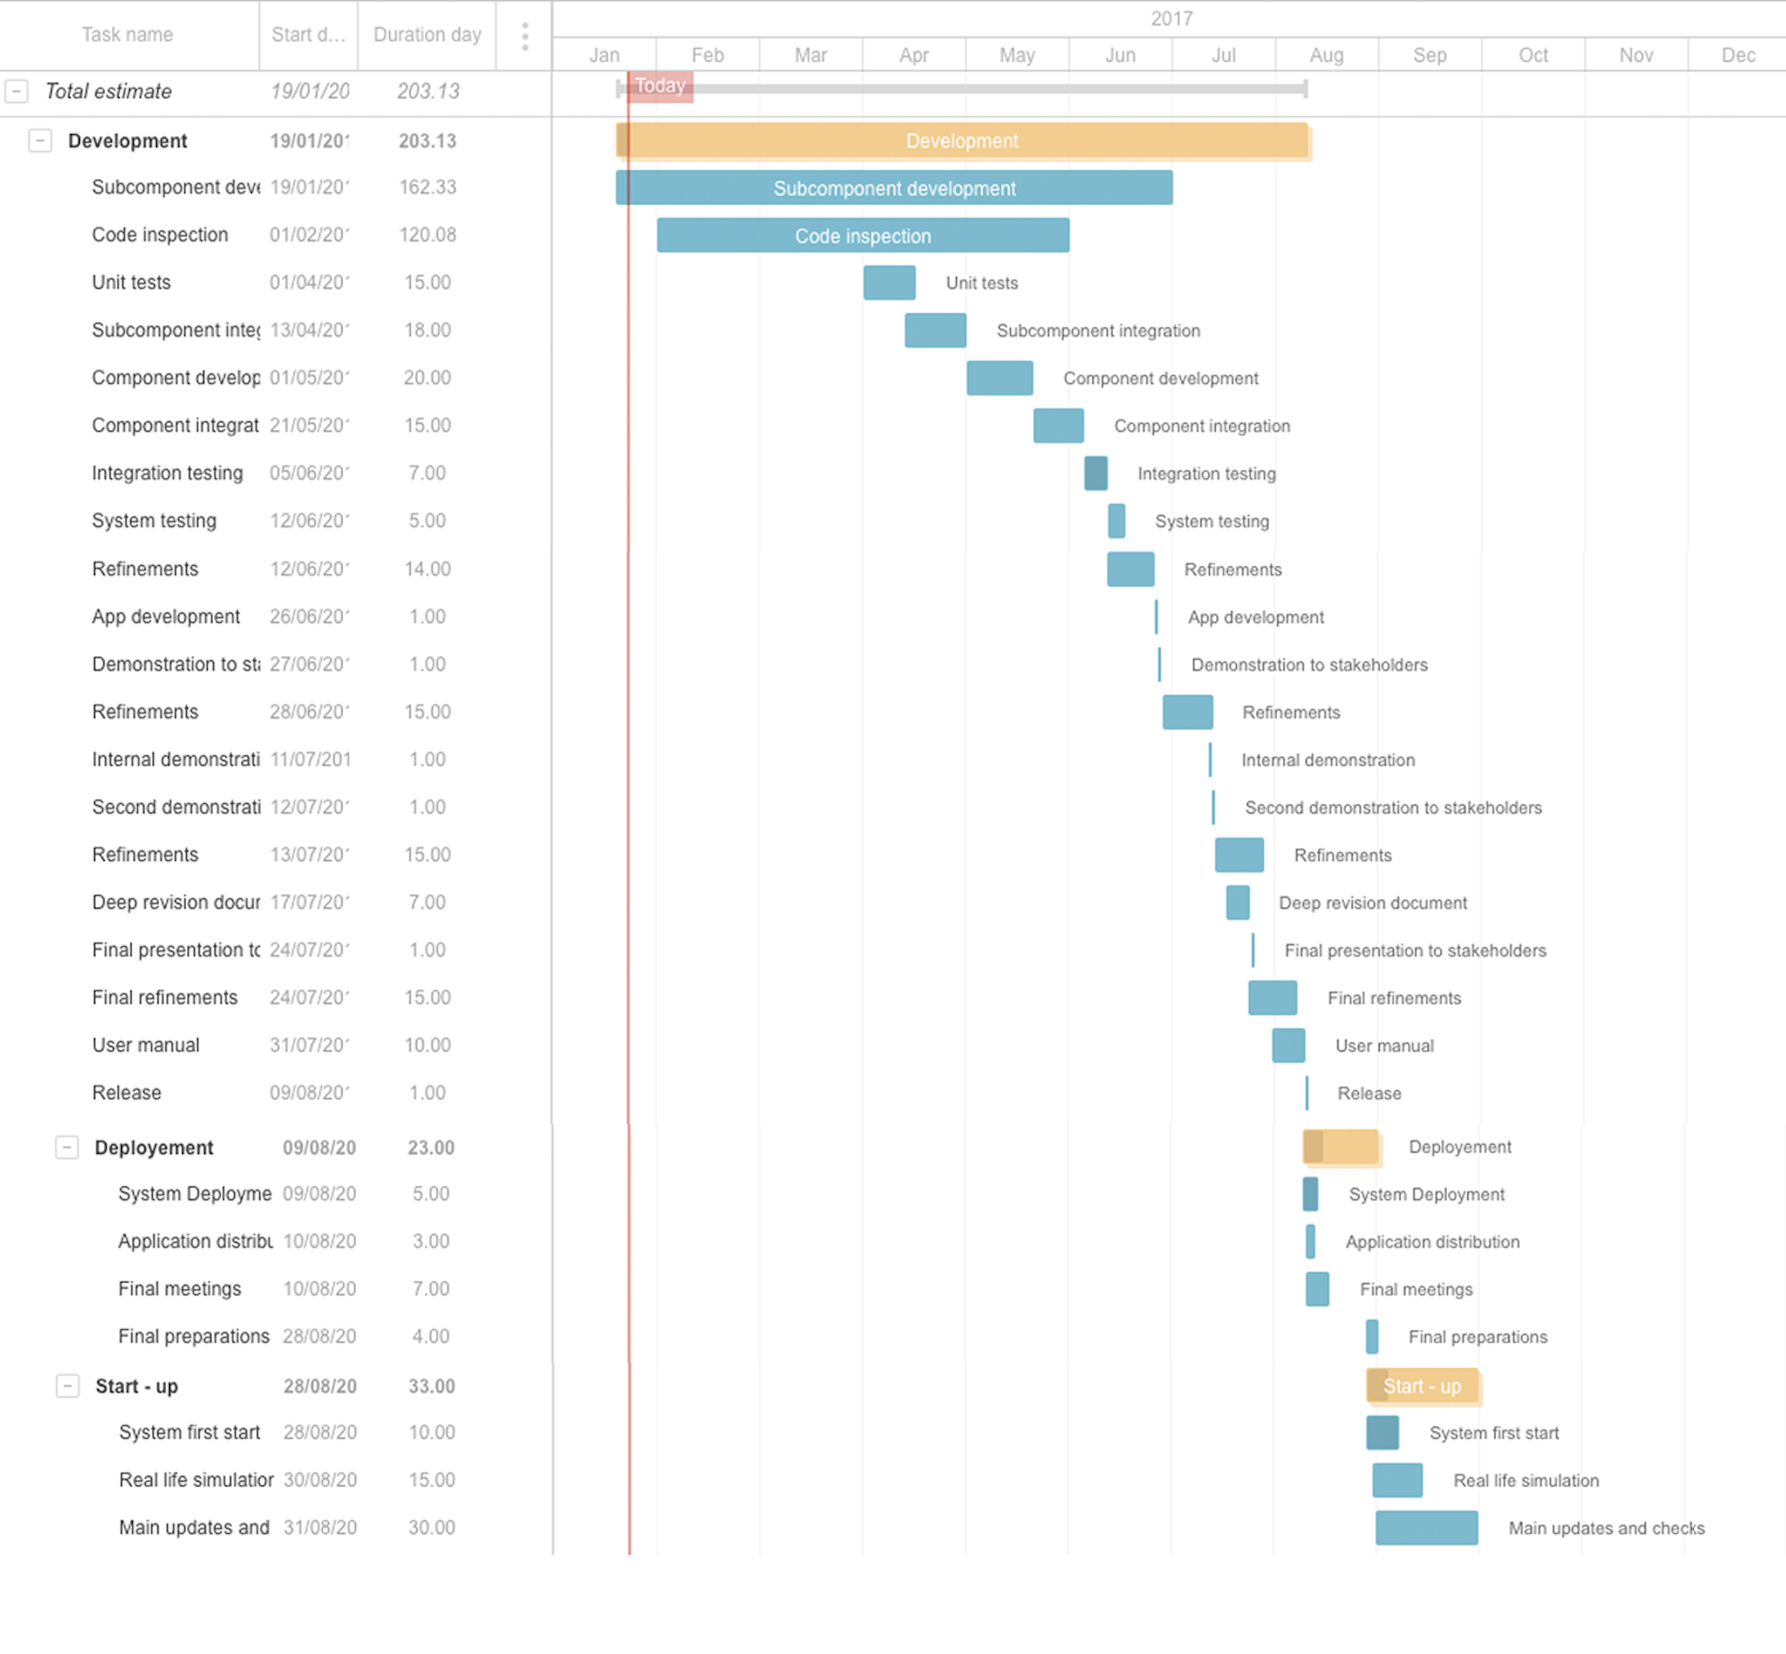
\includegraphics[scale=0.50]{Resources/gant2.png}
  \end{figure}\FloatBarrier
  \clearpage\section{Resource Allocation}
  In this chapter we are going to attach an outline of how the tasks defined in the schedule that is given in the previous section 
  have been splitted between the two members of the development team.  This document must be considered only as a general
  overview, and more detailed schedules will be produced during the the project to specify in major detail the organization 
  and split of the work in each of the development phases. The diagram is split in two parts because of its size and because 
  from the development phase on, the development of the project will be assigned to an external development team, which differs
  from the team that is working on the project at the moment.
    \begin{figure}[!h]
  \centering
    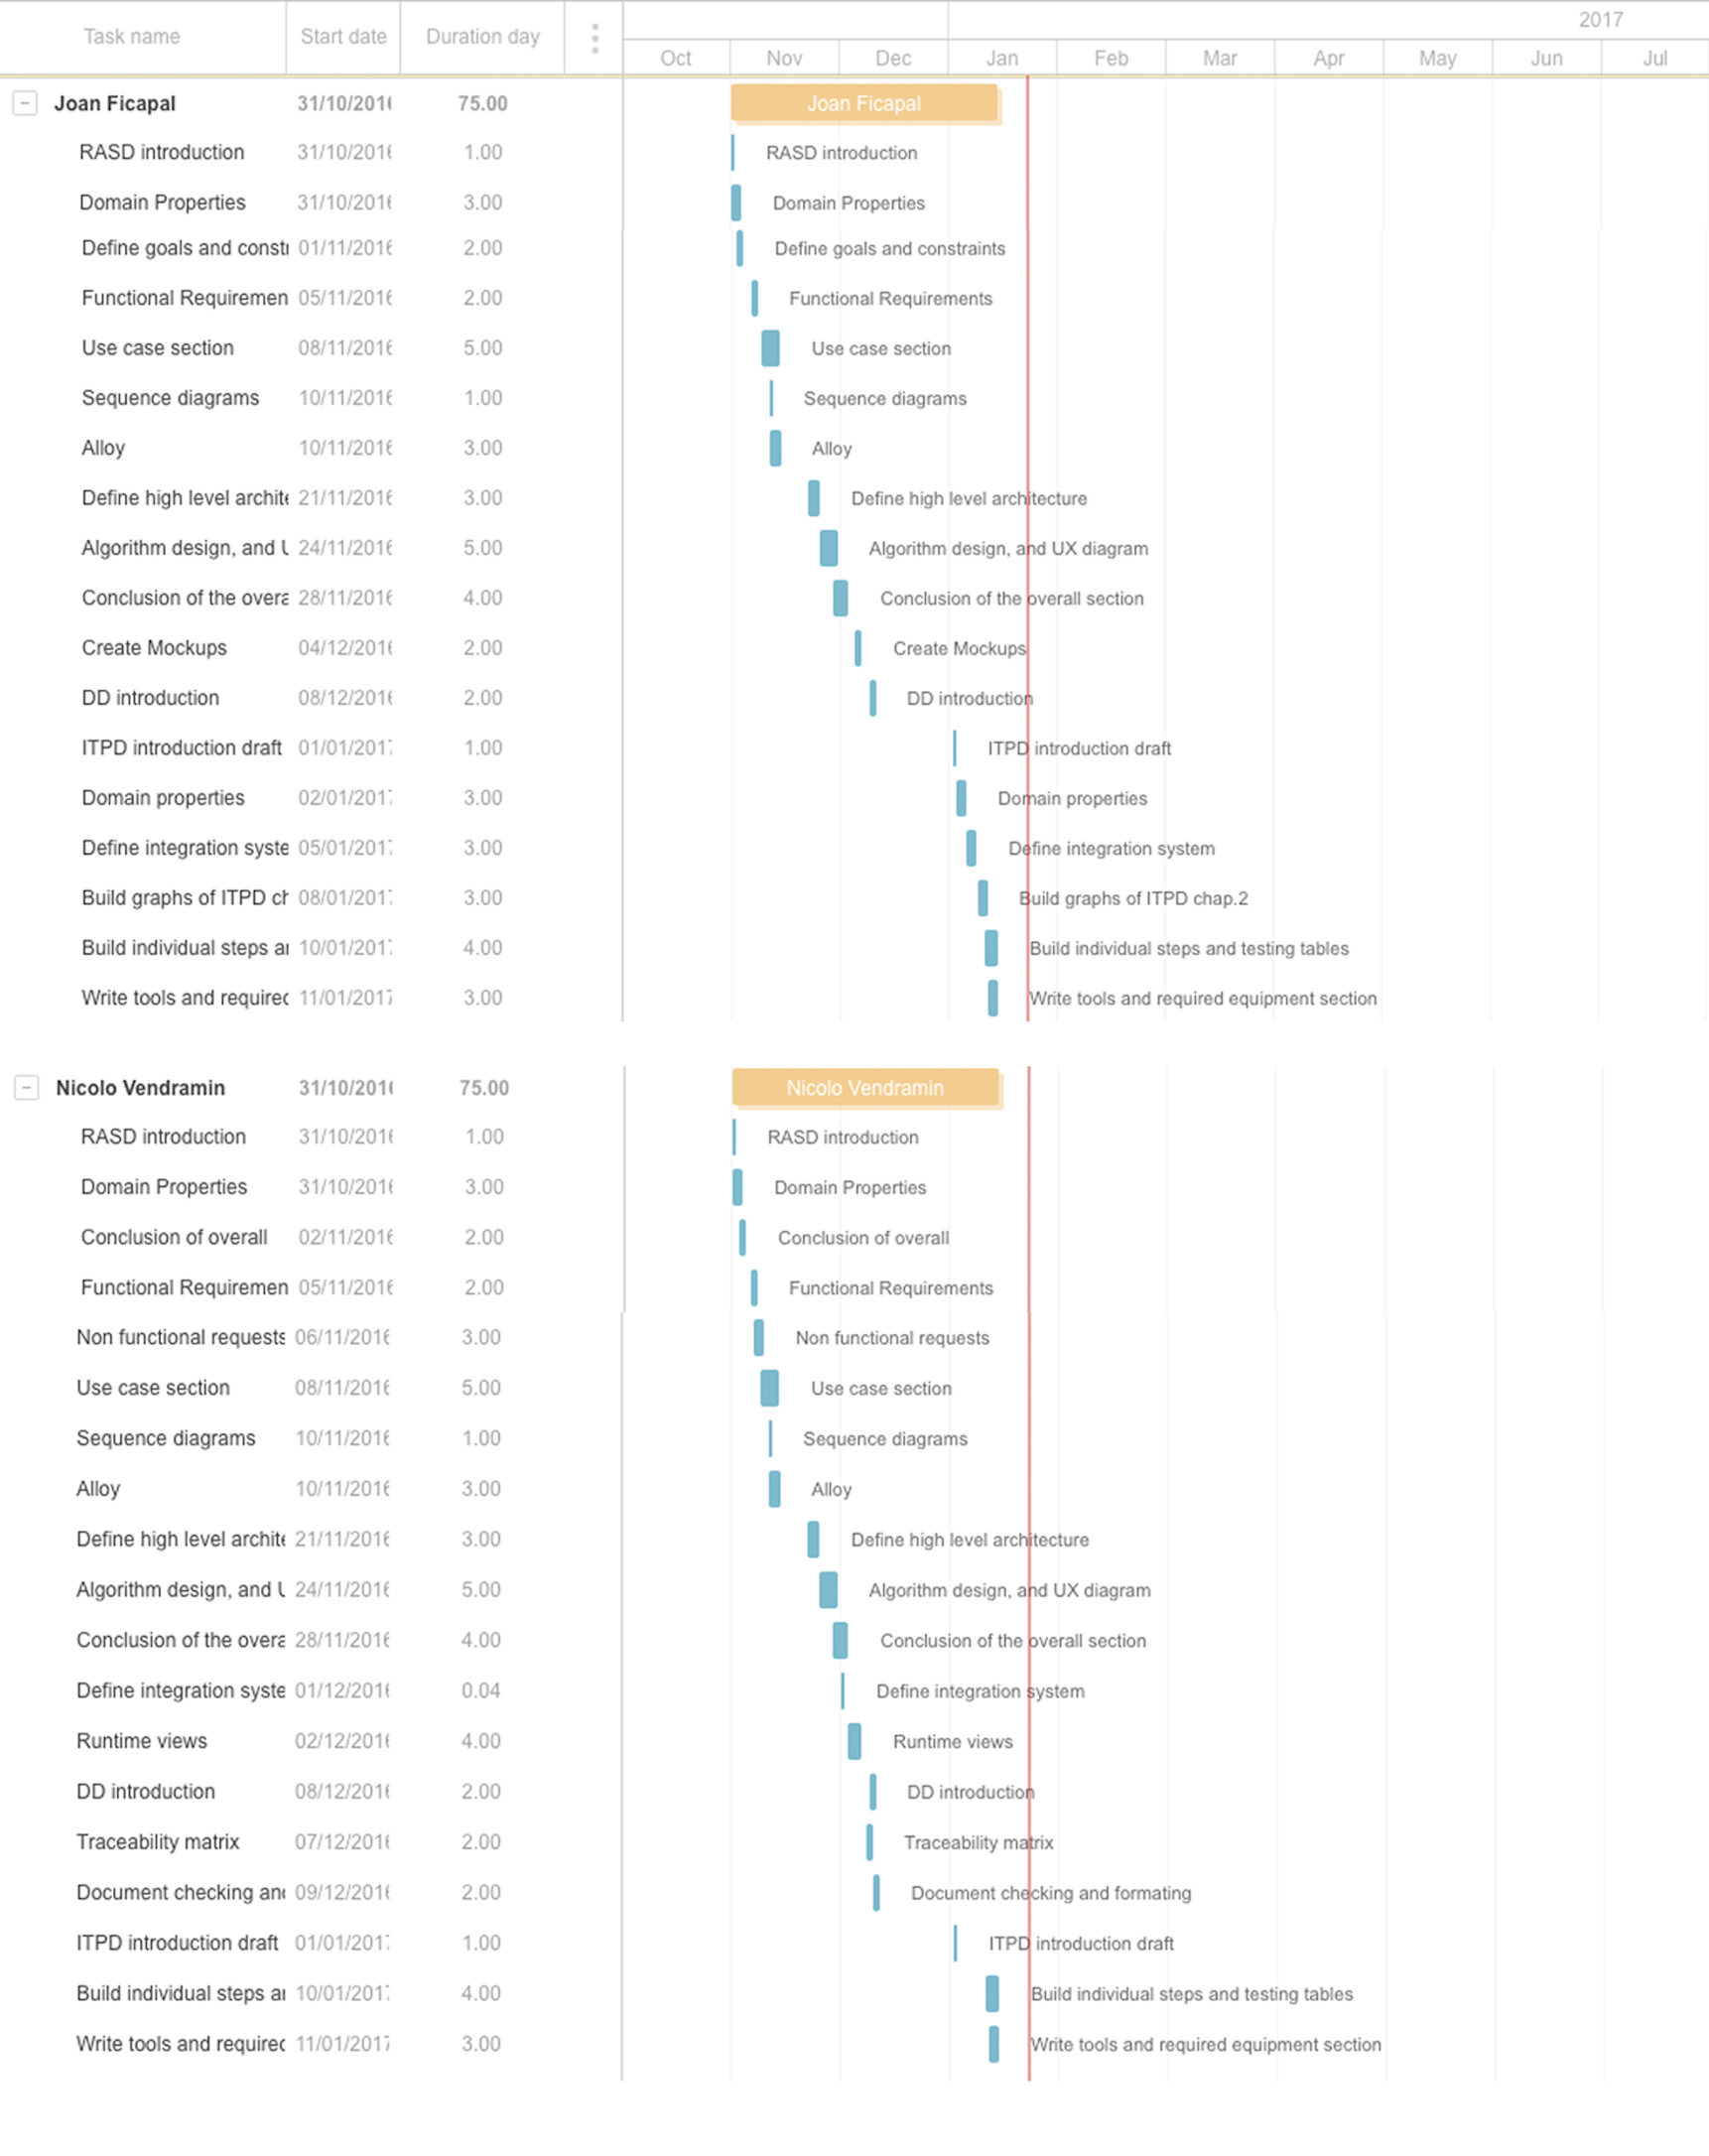
\includegraphics[scale=0.50]{Resources/scheduleJoanico.png}
  \end{figure}\FloatBarrier
      \begin{figure}[!h]
  \centering
    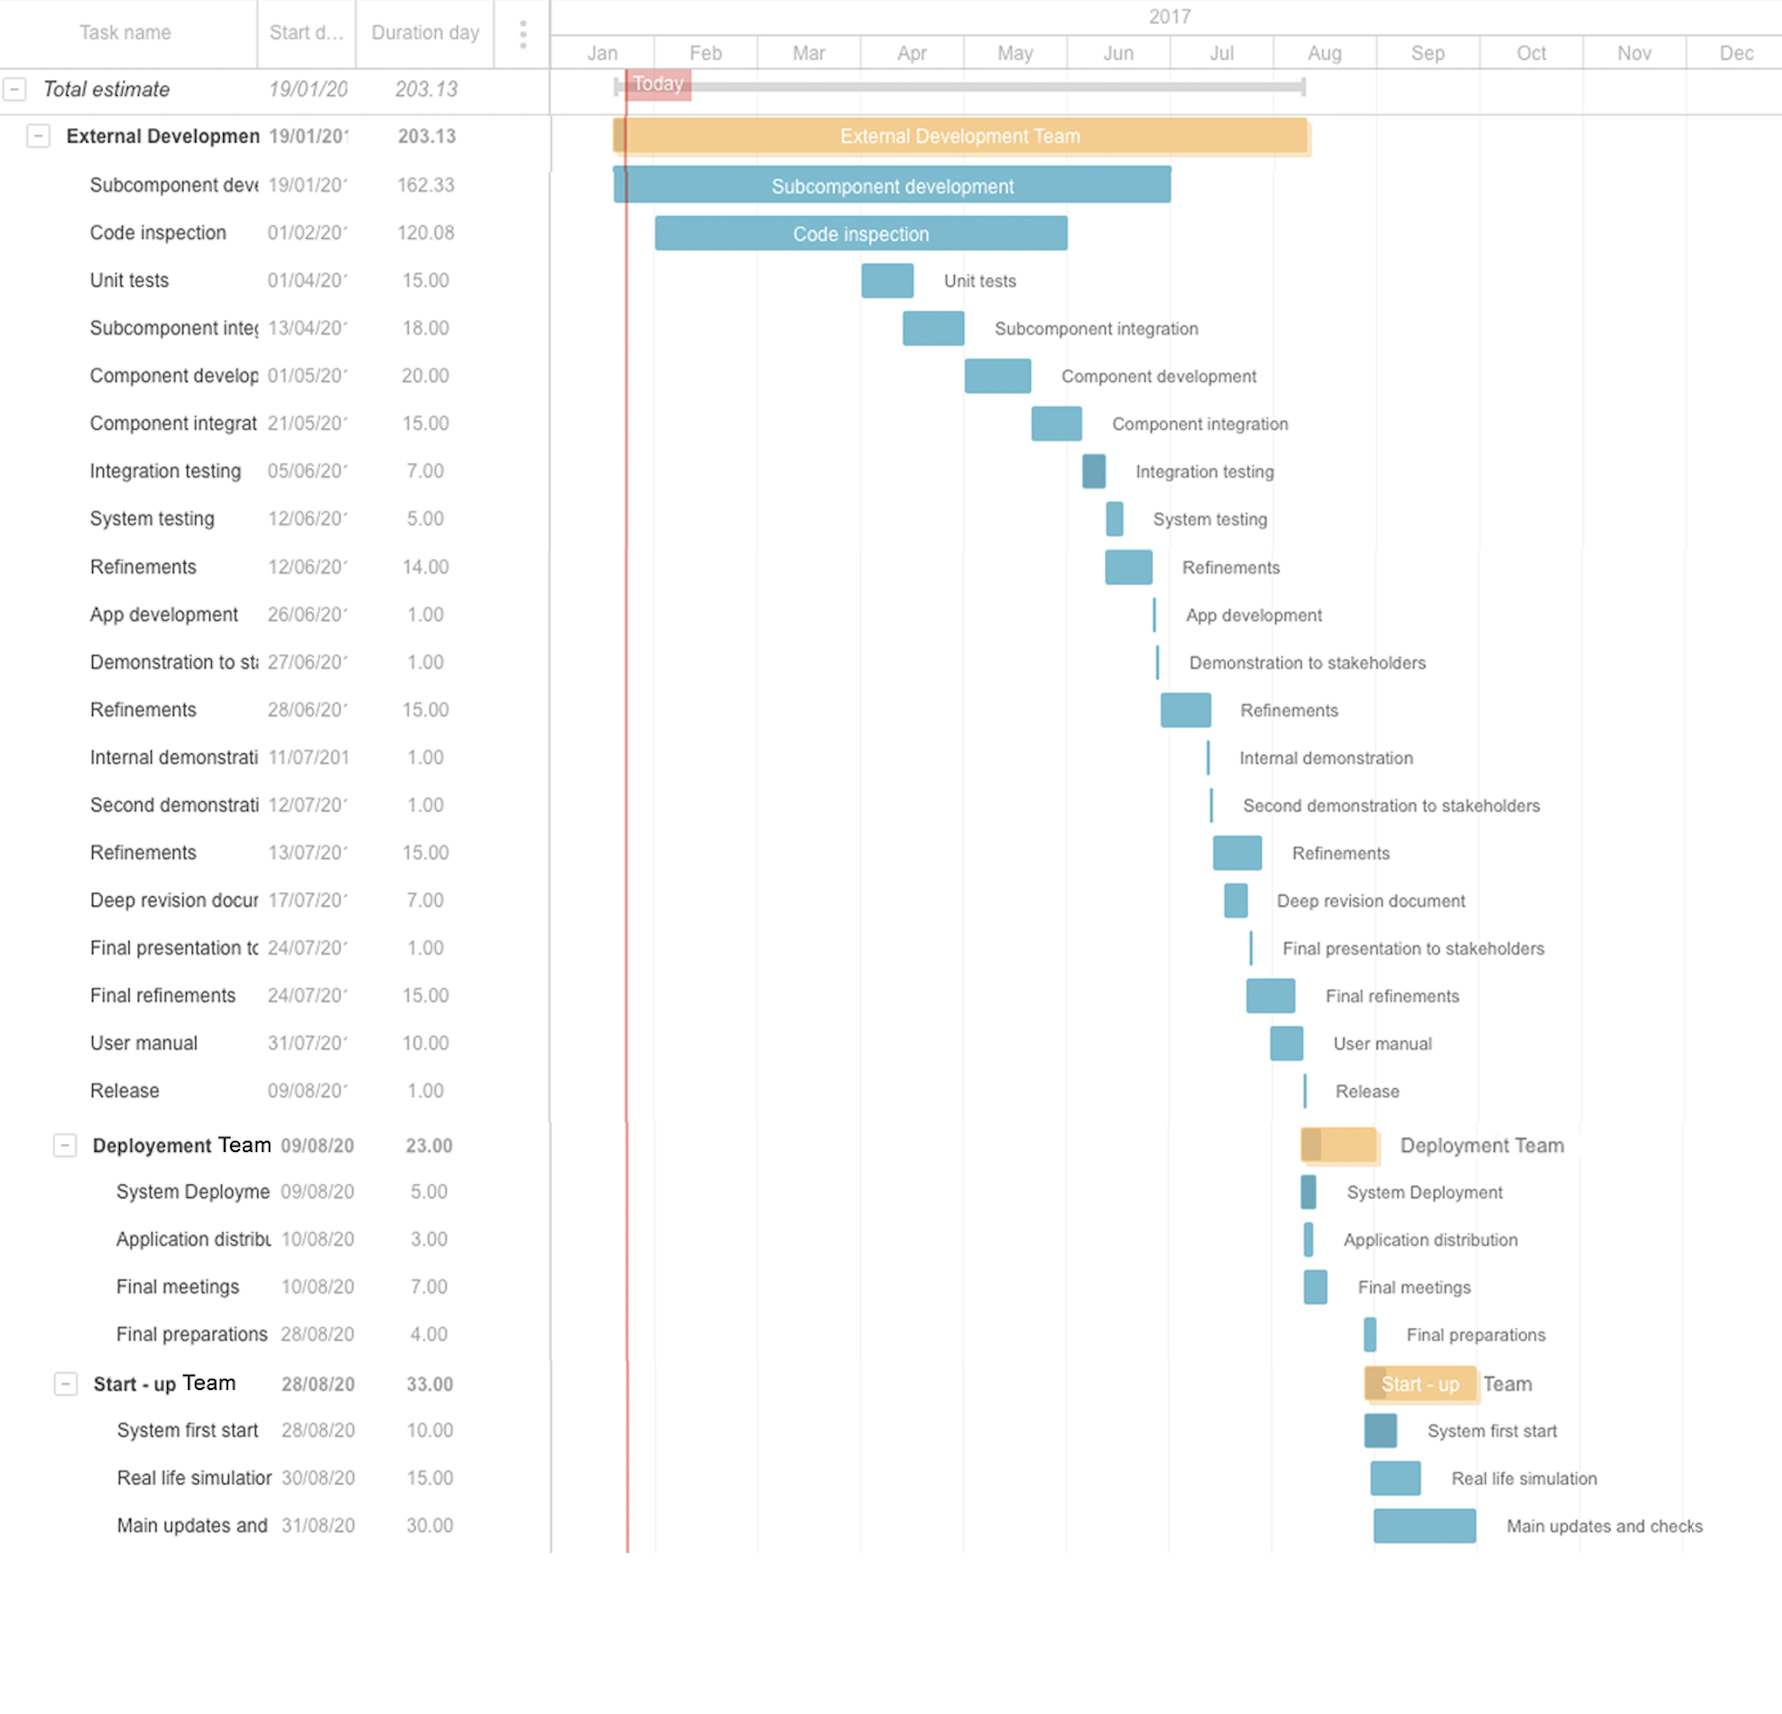
\includegraphics[scale=0.50]{Resources/ggdas.png}
  \end{figure}\FloatBarrier
  \clearpage\section{Risk Management}
  In these section we are going to outline which are the main risks that the development of the PowerEnjoy project may face.
  \\Generally speaking the problems that we could face can be grouped in x groups:
   \begin{description}
    \item[$\bullet$] Problems with the staff
    \item[$\bullet$] Problems with the stakeholders
    \item[$\bullet$] Technical Problems
    \item[$\bullet$] Managerial Problems
    \item[$\bullet$] Non Forecastable events affecting the evolution of the project.
  \end{description}
  Problems belonging to the first category are mainly due to the strong turnover that the personnel working on the project could suffer.
  This turnover is caused by the fact that the development of the project will be assigned to a group of developer selected on purpose that 
 may need some time to integrate in the project, causing in that way delays on the planned schedule, and also by the fact that the job-market
 in the field of IT is a quite dynamic market and exists the concrete possibility that some members of the staff leave the company.
 With managerial problems we refer to the ineptitude of the managers leading the team in the different phases of development (from the 
  elicitiation to the deployment and maintenance of the project). A bad attitude of the team leader could affect all the team, causing delays,
  an inefficient use of resources and possibly a bad working environment.\\
 The second category is wide in the sense that the stakeholders of the project are many and the possible problems that it could face because of 
 them. We are going to list the main ones, along with a quick explenation:
 \begin{description}
    \item[$\bullet$] Customer not interested in the project: even if some studies about the attractiveness of the applications
    have been done before the project was commissioned, a small, but not insignificant, probability that the final customer won't like 
    the service is still to be considered.
    \item[$\bullet$] Problems with direct competitors: we know that in the same market, some companies are already operating with profit. Even 
    if in this kind of market a new service can be seen by the client as an apprecciated integration of the coverage provided by the other
    services, is as well true that the presence of incumbents well-established in the market could cause a scarse interest in the client. 
    In addition the incumbents could apply some moves to make sure that the project fails without affecting their business.
    \item[$\bullet$] Problems with indirect competitors: with indirect competitors (e.g.: Public Transportation,
    bike-sharing services, the taxi service...) it could happen that in order to preserve their business they try to make pressure
    on the local governance in order to reduce the gap between them and the car-sharing service, affecting in this way the possible success
    of the PowerEnjoy project.
    \item[$\bullet$] Problems in the relationship with the local governance: in order to run the service, permissions and sponsorship 
    must be granted by the local governance of the city. In case the relationship goes wrong for any possible reason the project could
    suffer for delays in the schedule, due to the non-collaboration of the local authorities.
  \end{description}
  In order to avoid problems with the stakeholders in general is suggested to try to include them in the process of development of the project
  so that the relationship with them will be kept in the best possible way.\\
  The third possible category is the one concerning technical problems. The main possible problem is connected to the functioning
  and battery-duration of the cars used to provide the service. In case the vehicles chosen to be employed in the service are not sufficiently
  good the service would be perceived as non usefull, this being a problem for it.
  And finally the last category is mentioned to remind that the schedule could be affected as well by unforecastable events. 
\end{document}
